% Manuscript for the Journal of Statistics and Data Science in Sports (JSDSS): single-anonymous review
% (referees anonymous, authors named), PDF submission through OJS. Same sections, numbers, tables and
% figures as main.tex; only the front matter, availability statement and document class differ.
% Build: pdflatex main_jsdss -> bibtex main_jsdss -> pdflatex x2 (no journal style file needed).
\documentclass[11pt]{article}

\usepackage[utf8]{inputenc}
\usepackage[T1]{fontenc}
\usepackage[margin=1.1in]{geometry}
\usepackage[hidelinks]{hyperref}
\usepackage{lmodern}
\usepackage{microtype}
\usepackage{amsmath}
\usepackage{booktabs}
\usepackage{graphicx}
\usepackage{chngcntr}
\usepackage[section]{placeins}
\usepackage[round,authoryear]{natbib}
\bibpunct{(}{)}{;}{a}{}{,}
\usepackage{url}

% GENERATED by scripts/paper/make_numbers.py from paper/results/*.json - do not edit.
% One macro per quoted number, rounded as in paper/CLAIMS.md. Usable in text and math mode.

\newcommand{\CircuitSD}{0.0498}
\newcommand{\CircuitSDLo}{0.0354}
\newcommand{\CircuitSDHi}{0.0810}
\newcommand{\CircuitSDBootLo}{0.0284}
\newcommand{\CircuitSDBootHi}{0.0708}
\newcommand{\CircuitSDsPerTwenty}{1.00}
\newcommand{\CircuitSDsPerTwentyLo}{0.71}
\newcommand{\CircuitSDsPerTwentyHi}{1.62}
\newcommand{\CircuitLRStat}{220.8}
\newcommand{\CircuitBootP}{0.002}
\newcommand{\CircuitNBoot}{500}
\newcommand{\CircuitRange}{0.191}
\newcommand{\NCircuitsRaceFit}{13}
\newcommand{\NLapsRaceFit}{11{,}039}
\newcommand{\NRunsRaceFit}{820}
\newcommand{\NDriversRaceFit}{23}
\newcommand{\PooledNEvents}{82}
\newcommand{\PooledNCircuits}{23}
\newcommand{\PooledNRepeat}{20}
\newcommand{\PooledNLaps}{69{,}395}
\newcommand{\PooledNRuns}{4{,}445}
\newcommand{\PooledEventsPerCircuit}{4}
\newcommand{\PersistSD}{0.0278}
\newcommand{\PersistSDLo}{0.0197}
\newcommand{\PersistSDHi}{0.0405}
\newcommand{\PersistSDBootLo}{0.0157}
\newcommand{\PersistSDBootHi}{0.0380}
\newcommand{\EventSD}{0.0240}
\newcommand{\EventSDLo}{0.0208}
\newcommand{\EventSDHi}{0.0290}
\newcommand{\EventSDBootLo}{0.0191}
\newcommand{\EventSDBootHi}{0.0288}
\newcommand{\PersistShare}{0.57}
\newcommand{\PersistShareBootLo}{0.28}
\newcommand{\PersistShareBootHi}{0.75}
\newcommand{\PersistSDsPerTwenty}{0.56}
\newcommand{\PersistSDsPerTwentyLo}{0.39}
\newcommand{\PersistSDsPerTwentyHi}{0.81}
\newcommand{\EventSDsPerTwenty}{0.48}
\newcommand{\EventSDsPerTwentyLo}{0.42}
\newcommand{\EventSDsPerTwentyHi}{0.58}
\newcommand{\PooledLRCircuit}{27.0}
\newcommand{\PooledPCircuit}{0.002}
\newcommand{\PooledNBootCircuit}{500}
\newcommand{\PooledLREvent}{258.5}
\newcommand{\PooledRateCOne}{0.044}
\newcommand{\PooledRateCTwo}{0.043}
\newcommand{\PooledRateCThree}{0.060}
\newcommand{\PooledRateCFour}{0.066}
\newcommand{\PooledRateCFive}{0.073}
\newcommand{\PooledCompoundSD}{0.0134}
\newcommand{\PooledCompoundSDBootLo}{0.0111}
\newcommand{\PooledCompoundSDBootHi}{0.0156}
\newcommand{\PooledCompoundSDCorrHi}{0.0143}
\newcommand{\CircMinusCompound}{0.0137}
\newcommand{\CircMinusCompoundLo}{0.0022}
\newcommand{\CircMinusCompoundHi}{0.0253}
\newcommand{\CircGreaterCompoundP}{0.992}
\newcommand{\SensNoTwentyFiveCircuitSD}{0.0285}
\newcommand{\SensVerifiedCircuitSD}{0.0277}
\newcommand{\SensVerifiedNEvents}{80}
\newcommand{\RateCOne}{0.0410}
\newcommand{\RateCOneLo}{0.0079}
\newcommand{\RateCOneHi}{0.0742}
\newcommand{\RateCOneN}{55}
\newcommand{\RateCOneNLaps}{801}
\newcommand{\RateCTwo}{0.0373}
\newcommand{\RateCTwoLo}{0.0081}
\newcommand{\RateCTwoHi}{0.0665}
\newcommand{\RateCTwoN}{191}
\newcommand{\RateCTwoNLaps}{2{,}836}
\newcommand{\RateCThree}{0.0544}
\newcommand{\RateCThreeLo}{0.0258}
\newcommand{\RateCThreeHi}{0.0830}
\newcommand{\RateCThreeN}{242}
\newcommand{\RateCThreeNLaps}{3{,}316}
\newcommand{\RateCFour}{0.0633}
\newcommand{\RateCFourLo}{0.0346}
\newcommand{\RateCFourHi}{0.0921}
\newcommand{\RateCFourN}{223}
\newcommand{\RateCFourNLaps}{2{,}943}
\newcommand{\RateCFive}{0.0385}
\newcommand{\RateCFiveLo}{0.0090}
\newcommand{\RateCFiveHi}{0.0680}
\newcommand{\RateCFiveN}{109}
\newcommand{\RateCFiveNLaps}{1{,}143}
\newcommand{\ContrastCFiveCFour}{\ensuremath{-}0.0248}
\newcommand{\ContrastCFiveCFourLo}{\ensuremath{-}0.0332}
\newcommand{\ContrastCFiveCFourHi}{\ensuremath{-}0.0164}
\newcommand{\WithinEventTrend}{\ensuremath{-}0.0010}
\newcommand{\WithinEventTrendLo}{\ensuremath{-}0.0047}
\newcommand{\WithinEventTrendHi}{\ensuremath{+}0.0028}
\newcommand{\TrendSeasonTwentyTwo}{\ensuremath{+}0.0238}
\newcommand{\TrendSeasonTwentyTwoLo}{\ensuremath{+}0.0201}
\newcommand{\TrendSeasonTwentyTwoHi}{\ensuremath{+}0.0274}
\newcommand{\TotalLossTwentyCOne}{0.82}
\newcommand{\TotalLossTwentyCFive}{0.77}
\newcommand{\NaiveCOne}{\ensuremath{-}0.035}
\newcommand{\FuelCorrCOne}{\ensuremath{+}0.034}
\newcommand{\DeconCOne}{\ensuremath{+}0.041}
\newcommand{\NaiveCTwo}{\ensuremath{+}0.201}
\newcommand{\FuelCorrCTwo}{\ensuremath{+}0.038}
\newcommand{\DeconCTwo}{\ensuremath{+}0.037}
\newcommand{\NaiveCThree}{\ensuremath{-}0.037}
\newcommand{\FuelCorrCThree}{\ensuremath{+}0.048}
\newcommand{\DeconCThree}{\ensuremath{+}0.054}
\newcommand{\NaiveCFour}{\ensuremath{+}0.016}
\newcommand{\FuelCorrCFour}{\ensuremath{+}0.033}
\newcommand{\DeconCFour}{\ensuremath{+}0.063}
\newcommand{\NaiveCFive}{\ensuremath{-}0.070}
\newcommand{\FuelCorrCFive}{\ensuremath{+}0.016}
\newcommand{\DeconCFive}{\ensuremath{+}0.039}
\newcommand{\AblGapCOne}{0.007}
\newcommand{\AblGapCThree}{0.006}
\newcommand{\FuelCoefficient}{0.033}
\newcommand{\WidthNoCircuitCThree}{0.15}
\newcommand{\WidthNoCircuitCOne}{0.43}
\newcommand{\WidthShippedCThree}{1.38}
\newcommand{\WidthShippedCOne}{1.32}
\newcommand{\LagOneCircuitModel}{0.36}
\newcommand{\LagOneShipped}{0.22}
\newcommand{\CovEightyLOCO}{0.667}
\newcommand{\CovEightyK}{24}
\newcommand{\CovEightyN}{36}
\newcommand{\CovEightyWilsonLo}{0.50}
\newcommand{\CovEightyWilsonHi}{0.80}
\newcommand{\CovNinetyFiveLOCO}{0.889}
\newcommand{\CovEightyNoCircuit}{0.389}
\newcommand{\CovEightySBC}{0.762}
\newcommand{\CovEightyLapLevel}{0.806}
\newcommand{\NRunsCOneCTwo}{246}
\newcommand{\MDERealCOneCTwo}{0.0190}
\newcommand{\MDERealCTwoCThree}{0.0131}
\newcommand{\MDERealCThreeCFour}{0.0111}
\newcommand{\MDERealCFourCFive}{0.0139}
\newcommand{\MDERealCOneCTwoCircLo}{0.0189}
\newcommand{\MDERealCOneCTwoCircHi}{0.0190}
\newcommand{\MDERealCOneCTwoStress}{0.0262}
\newcommand{\MDERealCOneCTwoRound}{0.02}
\newcommand{\NStintsBalanced}{832}
\newcommand{\MDEBalanced}{0.0080}
\newcommand{\MDEBalancedStress}{0.0111}
\newcommand{\MDESplit}{0.0781}
\newcommand{\MDESplitLo}{0.0558}
\newcommand{\MDESplitHi}{0.1265}
\newcommand{\MDESimRealCOneCTwo}{0.019}
\newcommand{\MDESimRealCOneCTwoLo}{0.0188}
\newcommand{\MDESimRealCOneCTwoHi}{0.0196}
\newcommand{\MDESimRealCOneCTwoT}{0.023}
\newcommand{\MDESimReps}{1{,}000}
\newcommand{\PowerEffectSize}{0.006}
\newcommand{\PowerStintsCappello}{3}
\newcommand{\PXRunsBalSix}{1{,}489}
\newcommand{\PXRunsRealSix}{2{,}482}
\newcommand{\PXSplitCeilSix}{0.055}
\newcommand{\PXRunsBalTen}{536}
\newcommand{\PXRunsRealTen}{893}
\newcommand{\PXSplitCeilTen}{0.065}
\newcommand{\PXRunsBalTwenty}{134}
\newcommand{\PXRunsRealTwenty}{223}
\newcommand{\PXSplitCeilTwenty}{0.112}
\newcommand{\PXRunsBalThirty}{60}
\newcommand{\PXRunsRealThirty}{99}
\newcommand{\PXSplitCeilThirty}{0.192}
\newcommand{\PXSplitCeilLoSDThirty}{0.333}
\newcommand{\PXSimRunsBalTwenty}{138}
\newcommand{\PXSimRunsBalTwentyLo}{128}
\newcommand{\PXSimRunsBalTwentyHi}{147}
\newcommand{\PXSimRunsRealTwenty}{220}
\newcommand{\PXSimRunsRealTwentyLo}{210}
\newcommand{\PXSimRunsRealTwentyHi}{233}
\newcommand{\PXSimReps}{1{,}000}
\newcommand{\PXSizeBal}{0.056}
\newcommand{\PXSizeTBal}{0.032}
\newcommand{\PXSizeReal}{0.050}
\newcommand{\PXSizeTReal}{0.011}
\newcommand{\PXSizeReps}{2{,}000}
\newcommand{\PXSizeMCSE}{0.005}
\newcommand{\RaceToPracticeRatio}{0.56}
\newcommand{\RaceToPracticeRatioLo}{0.36}
\newcommand{\RaceToPracticeRatioHi}{0.81}
\newcommand{\NMatchedCellsMS}{82}
\newcommand{\LevelGapMS}{\ensuremath{-}0.0564}
\newcommand{\LevelGapMSLo}{\ensuremath{-}0.096}
\newcommand{\LevelGapMSHi}{\ensuremath{-}0.019}
\newcommand{\MatchedRaceSlopeMS}{0.0710}
\newcommand{\MatchedPracticeSlopeMS}{0.1274}
\newcommand{\NMatchedCellsAll}{105}
\newcommand{\NMatchedEventSeasons}{67}
\newcommand{\LevelGapAll}{\ensuremath{-}0.0586}
\newcommand{\LevelGapAllLo}{\ensuremath{-}0.093}
\newcommand{\LevelGapAllHi}{\ensuremath{-}0.024}
\newcommand{\RaceToPracticeRatioAll}{0.53}
\newcommand{\GapHard}{\ensuremath{-}0.056}
\newcommand{\GapMedium}{\ensuremath{-}0.038}
\newcommand{\GapSoft}{\ensuremath{-}0.080}
\newcommand{\StartAgeGapMS}{\ensuremath{-}0.0994}
\newcommand{\StartAgeGapMSLo}{\ensuremath{-}0.154}
\newcommand{\StartAgeGapMSHi}{\ensuremath{-}0.050}
\newcommand{\StartAgeRatioMS}{0.38}
\newcommand{\StartAgeRatioMSLo}{0.12}
\newcommand{\StartAgeRatioMSHi}{0.62}
\newcommand{\StartAgeCellsMS}{76}
\newcommand{\StartAgeCellsAll}{97}
\newcommand{\StartAgeEventSeasons}{60}
\newcommand{\IntersectGapMS}{\ensuremath{-}0.0578}
\newcommand{\IntersectGapMSLo}{\ensuremath{-}0.106}
\newcommand{\IntersectGapMSHi}{\ensuremath{-}0.012}
\newcommand{\IntersectRatioMS}{0.61}
\newcommand{\IntersectRatioMSLo}{0.39}
\newcommand{\IntersectRatioMSHi}{0.90}
\newcommand{\IntersectCellsMS}{48}
\newcommand{\IntersectCellsAll}{56}
\newcommand{\IntersectEventSeasons}{48}
\newcommand{\UnmatchedRatioMS}{0.43}
\newcommand{\UnmatchedGapMS}{\ensuremath{-}0.079}
\newcommand{\NUnmatchedCellsMS}{118}
\newcommand{\PlaceboGapMS}{\ensuremath{-}0.006}
\newcommand{\PlaceboGapMSLo}{\ensuremath{-}0.053}
\newcommand{\PlaceboGapMSHi}{\ensuremath{+}0.037}
\newcommand{\NPlaceboCellsMS}{63}
\newcommand{\NPlaceboCells}{76}
\newcommand{\PlaceboAdjGapMS}{\ensuremath{-}0.050}
\newcommand{\PlaceboAdjGapMSLo}{\ensuremath{-}0.106}
\newcommand{\PlaceboAdjGapMSHi}{\ensuremath{+}0.007}
\newcommand{\PlaceboShareMS}{0.11}
\newcommand{\RaceRunsStartAge}{1{,}411}
\newcommand{\RaceRunsStartAgeUsed}{416}
\newcommand{\RaceRunsStartAgeGap}{908}
\newcommand{\PracRunsStartAge}{407}
\newcommand{\PracRunsStartAgeUsed}{374}
\newcommand{\RaceUsedRuns}{563}
\newcommand{\RaceAllRuns}{2{,}770}
\newcommand{\PracUsedRuns}{858}
\newcommand{\PracAllRuns}{968}
\newcommand{\ReconWithinRunAll}{\ensuremath{+}0.009}
\newcommand{\ReconWithinRunAllLo}{\ensuremath{-}0.003}
\newcommand{\ReconWithinRunAllHi}{\ensuremath{+}0.021}
\newcommand{\ReconWithinRunTwentySix}{\ensuremath{-}0.002}
\newcommand{\ReconCrossSectionalAll}{\ensuremath{-}0.044}
\newcommand{\ReconFieldDemeanedAll}{\ensuremath{-}0.026}
\newcommand{\DidTWFESoftHard}{\ensuremath{-}0.0706}
\newcommand{\DidTWFESoftHardLo}{\ensuremath{-}0.134}
\newcommand{\DidTWFESoftHardHi}{\ensuremath{-}0.013}
\newcommand{\DidTWFESoftHardNEvents}{21}
\newcommand{\DidTWFESoftHardPPerm}{0.028}
\newcommand{\DidTWFESoftMedium}{\ensuremath{-}0.0055}
\newcommand{\DidTWFESoftMediumLo}{\ensuremath{-}0.048}
\newcommand{\DidTWFESoftMediumHi}{\ensuremath{+}0.035}
\newcommand{\DidTWFESoftMediumNEvents}{32}
\newcommand{\DidTWFESoftMediumPPerm}{0.807}
\newcommand{\DidTWFEMediumHard}{\ensuremath{-}0.0398}
\newcommand{\DidTWFEMediumHardLo}{\ensuremath{-}0.085}
\newcommand{\DidTWFEMediumHardHi}{\ensuremath{+}0.005}
\newcommand{\DidTWFEMediumHardNEvents}{31}
\newcommand{\DidTWFEMediumHardPPerm}{0.091}
\newcommand{\DidTWFESoftHardHolmP}{0.085}
\newcommand{\DidTWFESoftHardRaceContrast}{\ensuremath{+}0.018}
\newcommand{\DidTWFESoftMediumHolmP}{0.807}
\newcommand{\DidTWFESoftMediumRaceContrast}{\ensuremath{+}0.018}
\newcommand{\DidTWFEMediumHardHolmP}{0.182}
\newcommand{\DidTWFEMediumHardRaceContrast}{\ensuremath{+}0.018}
\newcommand{\UniformDampingImplied}{\ensuremath{-}0.019}
\newcommand{\UniformDampingObserved}{\ensuremath{-}0.028}
\newcommand{\PlaceboSoftMedium}{\ensuremath{-}0.124}
\newcommand{\PlaceboSoftMediumLo}{\ensuremath{-}0.207}
\newcommand{\PlaceboSoftMediumHi}{\ensuremath{-}0.033}
\newcommand{\NursingTrend}{\ensuremath{-}0.0280}
\newcommand{\NursingTrendLo}{\ensuremath{-}0.063}
\newcommand{\NursingTrendHi}{\ensuremath{+}0.014}
\newcommand{\NursingPOneSided}{0.070}
\newcommand{\NursingPTwoSided}{0.137}
\newcommand{\NursingMDE}{0.060}
\newcommand{\MultiverseSpecs}{74}
\newcommand{\MultiverseNegative}{70}
\newcommand{\MultiverseExcludesZero}{37}
\newcommand{\TelePrimaryEvents}{26}
\newcommand{\TelePrimaryLaps}{25{,}045}
\newcommand{\TeleExtensionEvents}{34}
\newcommand{\TelePrimarySlope}{\ensuremath{+}0.039}
\newcommand{\TelePrimarySlopeLo}{\ensuremath{-}0.130}
\newcommand{\TelePrimarySlopeHi}{\ensuremath{+}0.186}
\newcommand{\TelePrimaryPOneSided}{0.298}
\newcommand{\TelePrimaryPTwoSided}{0.595}
\newcommand{\TelePrimaryNEventsTrend}{14}
\newcommand{\TeleExtensionSlope}{\ensuremath{-}0.221}
\newcommand{\TeleExtensionSlopeLo}{\ensuremath{-}0.443}
\newcommand{\TeleExtensionSlopeHi}{\ensuremath{+}0.007}
\newcommand{\TeleExtensionPOneSided}{0.958}
\newcommand{\TeleExtensionPTwoSided}{0.084}
\newcommand{\TeleExtensionNEventsTrend}{16}
\newcommand{\HoldoutCells}{70}
\newcommand{\HoldoutWeekends}{44}
\newcommand{\FrozenFactor}{0.349}
\newcommand{\MaeScalar}{0.0355}
\newcommand{\MaeScalarLo}{0.0286}
\newcommand{\MaeScalarHi}{0.0426}
\newcommand{\MaeNaive}{0.112}
\newcommand{\MaeNaiveLo}{0.092}
\newcommand{\MaeNaiveHi}{0.132}
\newcommand{\MaeZero}{0.0502}
\newcommand{\MaeConstant}{0.0311}
\newcommand{\MaeStack}{0.0317}
\newcommand{\MaeShrink}{0.0295}
\newcommand{\DiffScalarVsConstant}{\ensuremath{+}0.0045}
\newcommand{\DiffScalarVsConstantLo}{\ensuremath{-}0.0044}
\newcommand{\DiffScalarVsConstantHi}{\ensuremath{+}0.0136}
\newcommand{\DiffScalarVsHistory}{\ensuremath{-}0.0039}
\newcommand{\DiffScalarVsHistoryLo}{\ensuremath{-}0.0149}
\newcommand{\DiffScalarVsHistoryHi}{\ensuremath{+}0.0072}
\newcommand{\DiffScalarVsStack}{\ensuremath{+}0.0039}
\newcommand{\DiffScalarVsStackLo}{\ensuremath{-}0.0053}
\newcommand{\DiffScalarVsStackHi}{\ensuremath{+}0.0130}
\newcommand{\MaeTwentySixScalar}{0.0561}
\newcommand{\MaeTwentySixNaive}{0.0871}
\newcommand{\MaeNested}{0.0595}
\newcommand{\NestedOptimism}{0.0035}
\newcommand{\TwentySixCells}{21}
\newcommand{\MaePooled}{0.0468}
\newcommand{\MaeHistory}{0.0394}
\newcommand{\MaeCompound}{0.0634}
\newcommand{\MaeZeroLo}{0.0418}
\newcommand{\MaeZeroHi}{0.0590}
\newcommand{\MaeConstantLo}{0.0246}
\newcommand{\MaeConstantHi}{0.0383}
\newcommand{\MaePooledLo}{0.0384}
\newcommand{\MaePooledHi}{0.0556}
\newcommand{\MaeHistoryLo}{0.0314}
\newcommand{\MaeHistoryHi}{0.0480}
\newcommand{\MaeCompoundLo}{0.0504}
\newcommand{\MaeCompoundHi}{0.0771}
\newcommand{\MaeShrinkLo}{0.0245}
\newcommand{\MaeShrinkHi}{0.0348}
\newcommand{\MaeStackLo}{0.0255}
\newcommand{\MaeStackHi}{0.0382}
\newcommand{\PitLossGreen}{22.50}
\newcommand{\PitLossGreenLo}{22.06}
\newcommand{\PitLossGreenHi}{22.97}
\newcommand{\PitStopsGreen}{2{,}426}
\newcommand{\PitRacesGreen}{103}
\newcommand{\PitRatioVSC}{0.930}
\newcommand{\PitRatioVSCLo}{0.81}
\newcommand{\PitRatioVSCHi}{1.09}
\newcommand{\PitStopsVSC}{235}
\newcommand{\PitRatioSC}{0.883}
\newcommand{\PitRatioSCLo}{0.67}
\newcommand{\PitRatioSCHi}{1.12}
\newcommand{\PitStopsSC}{348}
\newcommand{\PitRacesSC}{40}
\newcommand{\PitRatioYellow}{1.159}
\newcommand{\PitRatioVSCTwentySix}{1.068}
\newcommand{\PitRatioSCTwentySix}{1.597}
\newcommand{\PitRatioSCNoFilter}{1.11}
\newcommand{\PitSCOutsideFilter}{119}
\newcommand{\PitConsoleFraction}{0.883}
\newcommand{\PitRatioSCNoFilterLo}{0.79}
\newcommand{\PitRatioSCNoFilterHi}{1.99}
\newcommand{\StratRacesOOT}{38}
\newcommand{\StratDiffLapRule}{\ensuremath{+}0.158}
\newcommand{\StratDiffLapRuleLo}{\ensuremath{+}0.000}
\newcommand{\StratDiffLapRuleHi}{\ensuremath{+}0.316}
\newcommand{\StratDiffAlwaysOne}{\ensuremath{+}0.289}
\newcommand{\StratDiffAlwaysOneLo}{\ensuremath{+}0.053}
\newcommand{\StratDiffAlwaysOneHi}{\ensuremath{+}0.526}
\newcommand{\StratProductMatches}{8}
\newcommand{\StratProductOf}{13}
\newcommand{\StratAlwaysOneMatches}{5}
\newcommand{\StratAlwaysOneOf}{13}
\newcommand{\StratRuleThreshold}{58}
\newcommand{\StratRuleMatches}{10}
\newcommand{\StratRuleOf}{13}
\newcommand{\StratLOROLapRule}{\ensuremath{+}0.073}
\newcommand{\StratLOROLapRuleLo}{\ensuremath{-}0.073}
\newcommand{\StratLOROLapRuleHi}{\ensuremath{+}0.220}
\newcommand{\StratLORORaces}{41}
\newcommand{\TableThreeHard}{0.0546}
\newcommand{\TableThreeMedium}{0.0552}
\newcommand{\TableThreeHardPub}{0.054}
\newcommand{\TableThreeMediumPub}{0.060}
\newcommand{\PMediumGtHard}{0.528}
\newcommand{\FuelDefectKg}{4.74}
\newcommand{\PMediumGtHardCorrected}{0.539}
\newcommand{\FuelDefectDeltaCRPS}{\ensuremath{-}0.0013}
\newcommand{\BenchWinsVsRepoSSM}{2}
\newcommand{\BenchCRPSOurs}{0.326}
\newcommand{\BenchCRPSSSM}{0.220}
\newcommand{\BenchDiffSSM}{\ensuremath{+}0.106}
\newcommand{\BenchDiffSSMLo}{\ensuremath{+}0.067}
\newcommand{\BenchDiffSSMHi}{\ensuremath{+}0.146}
\newcommand{\BenchSignPSSM}{0.0074}
\newcommand{\BenchNRaces}{15}
\newcommand{\AustriaCRPSOurs}{0.229}
\newcommand{\AustriaCRPSTheirs}{0.2022}
\newcommand{\AustriaDiff}{\ensuremath{+}0.024}
\newcommand{\AustriaDiffLo}{\ensuremath{-}0.004}
\newcommand{\AustriaDiffHi}{\ensuremath{+}0.049}
\newcommand{\SkewTDelta}{\ensuremath{-}0.0066}
\newcommand{\SkewTBetter}{10}
\newcommand{\SkewTRaces}{12}
\newcommand{\SkewTAustriaDelta}{\ensuremath{-}0.0014}
\newcommand{\JournalRacesScored}{15}
\newcommand{\JournalRacesTotal}{19}
\newcommand{\JournalWinsSSM}{2}
\newcommand{\JournalCRPSSSM}{0.2203}
\newcommand{\JournalWinsAR}{5}
\newcommand{\JournalCRPSAR}{0.2809}
\newcommand{\JournalDiffAR}{\ensuremath{+}0.045}
\newcommand{\JournalDiffARLo}{\ensuremath{-}0.007}
\newcommand{\JournalDiffARHi}{\ensuremath{+}0.095}
\newcommand{\JournalSignPAR}{0.302}
\newcommand{\JournalRMSPESSM}{0.375}
\newcommand{\JournalRMSPEOurs}{0.524}
\newcommand{\JournalRMSPEAR}{0.456}
\newcommand{\JournalSSMBeatsARCommon}{14}
\newcommand{\JournalSSMBeatsARAll}{16}
\newcommand{\JournalPrintedMeanAR}{0.300}
\newcommand{\JournalMeanARAll}{0.2996}
\newcommand{\JournalAustriaAR}{0.289}
\newcommand{\JournalAustriaRMSPEAR}{1.478}
\newcommand{\JournalWinsRMSPESSM}{1}
\newcommand{\JournalWinsRMSPEAR}{5}
\newcommand{\KeepRunsDiff}{\ensuremath{-}0.0048}
\newcommand{\KeepRunsDiffLo}{\ensuremath{-}0.0076}
\newcommand{\KeepRunsDiffHi}{\ensuremath{-}0.0021}
\newcommand{\KeepRunsCommonCells}{69}
\newcommand{\WarmupDiff}{\ensuremath{-}0.0018}
\newcommand{\WarmupDiffLo}{\ensuremath{-}0.0056}
\newcommand{\WarmupDiffHi}{\ensuremath{+}0.0006}
\newcommand{\WarmupSignFlipP}{0.50}
\newcommand{\PracticeLapsShipped}{2{,}815}
\newcommand{\PracticeLapsLegacy}{2{,}339}
\newcommand{\NLapsCleanTwentySix}{23{,}856}
\newcommand{\NEventsInFileTwentySix}{14}
\newcommand{\NLapsSeasonTwentyTwo}{13{,}637}
\newcommand{\NEventsSeasonTwentyTwo}{18}
\newcommand{\NRunsSeasonTwentyTwo}{1{,}038}
\newcommand{\NLapsSeasonTwentyThree}{13{,}536}
\newcommand{\NEventsSeasonTwentyThree}{16}
\newcommand{\NRunsSeasonTwentyThree}{860}
\newcommand{\NLapsSeasonTwentyFour}{15{,}942}
\newcommand{\NEventsSeasonTwentyFour}{18}
\newcommand{\NRunsSeasonTwentyFour}{857}
\newcommand{\NLapsSeasonTwentyFive}{15{,}279}
\newcommand{\NEventsSeasonTwentyFive}{17}
\newcommand{\NRunsSeasonTwentyFive}{872}
\newcommand{\NLapsSeasonTwentySix}{11{,}039}
\newcommand{\NEventsSeasonTwentySix}{13}
\newcommand{\NRunsSeasonTwentySix}{820}
\newcommand{\SDDriverEvent}{1.15}
\newcommand{\SDRunIntercept}{0.30}
\newcommand{\SDRunSlope}{0.035}
\newcommand{\SDResidual}{0.55}
\newcommand{\CompoundRateSD}{0.0114}
\newcommand{\EngineRateDiff}{0.000004}
\newcommand{\CircuitSDSeasonTwentyTwo}{0.0412}
\newcommand{\CircuitSDSeasonTwentyThree}{0.0314}
\newcommand{\CircuitSDSeasonTwentyFour}{0.0252}
\newcommand{\CircuitSDSeasonTwentyFive}{0.0227}
\newcommand{\CircuitSDSeasonTwentySix}{0.0460}
\newcommand{\ReproCorr}{0.9997}
\newcommand{\ReproRaces}{12}
\newcommand{\TeleJoinFraction}{0.97}
\newcommand{\LevelGapMSAbs}{0.056}
\newcommand{\LevelGapMSAbsMin}{0.019}
\newcommand{\LevelGapMSAbsMax}{0.096}
\newcommand{\PersistSDAbs}{0.028}
\newcommand{\PersistSDLoAbs}{0.020}
\newcommand{\PersistSDHiAbs}{0.041}
\newcommand{\EventSDAbs}{0.024}
\newcommand{\RunSlopeSD}{0.0382}
\newcommand{\RunSlopeSDAbs}{0.038}
\newcommand{\PooledCompoundSDAbs}{0.013}
\newcommand{\MaeScalarAbs}{0.036}
\newcommand{\MaeConstantAbs}{0.031}
\newcommand{\PoolConTwoOne}{\ensuremath{-}0.002}
\newcommand{\PoolConTwoOneLo}{\ensuremath{-}0.006}
\newcommand{\PoolConTwoOneHi}{\ensuremath{+}0.003}
\newcommand{\PoolMDETwoOne}{0.007}
\newcommand{\PoolMDETTwoOne}{0.007}
\newcommand{\PoolConThreeTwo}{\ensuremath{+}0.017}
\newcommand{\PoolConThreeTwoLo}{\ensuremath{+}0.014}
\newcommand{\PoolConThreeTwoHi}{\ensuremath{+}0.020}
\newcommand{\PoolMDEThreeTwo}{0.005}
\newcommand{\PoolMDETThreeTwo}{0.005}
\newcommand{\PoolConFourThree}{\ensuremath{+}0.007}
\newcommand{\PoolConFourThreeLo}{\ensuremath{+}0.004}
\newcommand{\PoolConFourThreeHi}{\ensuremath{+}0.009}
\newcommand{\PoolMDEFourThree}{0.003}
\newcommand{\PoolMDETFourThree}{0.003}
\newcommand{\PoolConFiveFour}{\ensuremath{+}0.007}
\newcommand{\PoolConFiveFourLo}{\ensuremath{+}0.003}
\newcommand{\PoolConFiveFourHi}{\ensuremath{+}0.011}
\newcommand{\PoolMDEFiveFour}{0.006}
\newcommand{\PoolMDETFiveFour}{0.006}
\newcommand{\SixConTwoOne}{\ensuremath{-}0.004}
\newcommand{\SixConTwoOneLo}{\ensuremath{-}0.022}
\newcommand{\SixConTwoOneHi}{\ensuremath{+}0.014}
\newcommand{\SixMDETwoOne}{0.026}
\newcommand{\SixMDETTwoOne}{0.032}
\newcommand{\SixConThreeTwo}{\ensuremath{+}0.017}
\newcommand{\SixConThreeTwoLo}{\ensuremath{+}0.004}
\newcommand{\SixConThreeTwoHi}{\ensuremath{+}0.030}
\newcommand{\SixMDEThreeTwo}{0.019}
\newcommand{\SixMDETThreeTwo}{0.020}
\newcommand{\SixConFourThree}{\ensuremath{+}0.009}
\newcommand{\SixConFourThreeLo}{\ensuremath{+}0.003}
\newcommand{\SixConFourThreeHi}{\ensuremath{+}0.015}
\newcommand{\SixMDEFourThree}{0.009}
\newcommand{\SixMDETFourThree}{0.010}
\newcommand{\SixConFiveFour}{\ensuremath{-}0.025}
\newcommand{\SixConFiveFourLo}{\ensuremath{-}0.033}
\newcommand{\SixConFiveFourHi}{\ensuremath{-}0.016}
\newcommand{\SixMDEFiveFour}{0.012}
\newcommand{\SixMDETFiveFour}{0.013}
\newcommand{\MundlakPoolP}{0.48}
\newcommand{\MundlakPoolShiftOne}{\ensuremath{+}0.0004}
\newcommand{\MundlakPoolShiftTwo}{\ensuremath{+}0.0002}
\newcommand{\MundlakPoolShiftThree}{\ensuremath{+}0.0004}
\newcommand{\MundlakPoolShiftFour}{\ensuremath{+}0.0006}
\newcommand{\MundlakPoolShiftFive}{\ensuremath{+}0.0018}
\newcommand{\MundlakSixP}{0.62}
\newcommand{\MundlakSixShiftOne}{\ensuremath{+}0.0052}
\newcommand{\MundlakSixShiftTwo}{\ensuremath{+}0.0030}
\newcommand{\MundlakSixShiftThree}{\ensuremath{+}0.0018}
\newcommand{\MundlakSixShiftFour}{\ensuremath{+}0.0047}
\newcommand{\MundlakSixShiftFive}{\ensuremath{+}0.0037}
\newcommand{\ApproxPoolRateOne}{0.056}
\newcommand{\ApproxPoolRateTwo}{0.047}
\newcommand{\ApproxPoolRateThree}{0.058}
\newcommand{\ApproxPoolRateFour}{0.059}
\newcommand{\ApproxPoolRateFive}{0.053}
\newcommand{\ApproxPoolCompoundSD}{0.0047}
\newcommand{\ApproxSixRateOne}{0.082}
\newcommand{\ApproxSixRateTwo}{0.053}
\newcommand{\ApproxSixRateThree}{0.050}
\newcommand{\ApproxSixRateFour}{0.042}
\newcommand{\ApproxSixRateFive}{0.022}
\newcommand{\ApproxSixCompoundSD}{0.0219}
\newcommand{\ApproxPoolCircuitSD}{0.0247}
\newcommand{\PooledCompoundSDCorr}{0.0115}
\newcommand{\RecExactExoBias}{\ensuremath{+}0.000}
\newcommand{\RecExactExoCov}{0.92}
\newcommand{\RecExactMundlakExoBias}{\ensuremath{+}0.000}
\newcommand{\RecExactMundlakExoCov}{0.92}
\newcommand{\RecApproxExoBias}{\ensuremath{+}0.002}
\newcommand{\RecApproxExoCov}{0.92}
\newcommand{\RecCrossExoBias}{\ensuremath{+}0.000}
\newcommand{\RecCrossExoCov}{0.79}
\newcommand{\RecFieldExoBias}{\ensuremath{+}0.000}
\newcommand{\RecFieldExoCov}{0.80}
\newcommand{\RecFuelExoBias}{\ensuremath{-}0.012}
\newcommand{\RecFuelExoCov}{0.42}
\newcommand{\RecNaiveExoBias}{\ensuremath{-}0.062}
\newcommand{\RecNaiveExoCov}{0.05}
\newcommand{\RecExactExoCircBias}{\ensuremath{-}0.0017}
\newcommand{\RecExactExoWorstCov}{0.89}
\newcommand{\RecExactPaceBias}{\ensuremath{-}0.001}
\newcommand{\RecExactPaceCov}{0.92}
\newcommand{\RecExactMundlakPaceBias}{\ensuremath{-}0.001}
\newcommand{\RecExactMundlakPaceCov}{0.92}
\newcommand{\RecApproxPaceBias}{\ensuremath{+}0.001}
\newcommand{\RecApproxPaceCov}{0.92}
\newcommand{\RecCrossPaceBias}{\ensuremath{-}0.027}
\newcommand{\RecCrossPaceCov}{0.51}
\newcommand{\RecFieldPaceBias}{\ensuremath{-}0.027}
\newcommand{\RecFieldPaceCov}{0.51}
\newcommand{\RecFuelPaceBias}{\ensuremath{-}0.012}
\newcommand{\RecFuelPaceCov}{0.43}
\newcommand{\RecNaivePaceBias}{\ensuremath{-}0.077}
\newcommand{\RecNaivePaceCov}{0.02}
\newcommand{\RecExactPaceCircBias}{\ensuremath{-}0.0018}
\newcommand{\RecExactPaceWorstCov}{0.87}
\newcommand{\RecExactWearBias}{\ensuremath{-}0.009}
\newcommand{\RecExactWearCov}{0.79}
\newcommand{\RecExactMundlakWearBias}{\ensuremath{-}0.008}
\newcommand{\RecExactMundlakWearCov}{0.81}
\newcommand{\RecApproxWearBias}{\ensuremath{-}0.007}
\newcommand{\RecApproxWearCov}{0.87}
\newcommand{\RecCrossWearBias}{\ensuremath{-}0.032}
\newcommand{\RecCrossWearCov}{0.32}
\newcommand{\RecFieldWearBias}{\ensuremath{-}0.035}
\newcommand{\RecFieldWearCov}{0.30}
\newcommand{\RecFuelWearBias}{\ensuremath{-}0.029}
\newcommand{\RecFuelWearCov}{0.22}
\newcommand{\RecNaiveWearBias}{\ensuremath{-}0.070}
\newcommand{\RecNaiveWearCov}{0.03}
\newcommand{\RecExactWearCircBias}{\ensuremath{-}0.0061}
\newcommand{\RecExactWearWorstCov}{0.72}
\newcommand{\RecExactWearBiasAbs}{0.009}
\newcommand{\NoTwentySixCircuitSD}{0.030}
\newcommand{\NoTwentySixEventSD}{0.019}
\newcommand{\NoTwentySixShare}{0.71}
\newcommand{\NoTwentySixCompoundSD}{0.019}
\newcommand{\NoTwentySixRateCFive}{0.091}
\newcommand{\NoTwentySixNEvents}{69}
\newcommand{\RecFuelExoBiasAbs}{0.012}
\newcommand{\RecTrueCircuitSD}{0.044}
\newcommand{\RecReps}{500}

\newcommand{\spl}{\,s/lap}
% Archived release of the repository; set to ", archived at \url{https://doi.org/...}" once Zenodo mints the DOI.
\newcommand{\ZenodoNote}{}

\title{What public timing data can tell us about tyre degradation in Formula~1}
\author{Akshat Gupta\\[2pt]
  \small School of AI and Computer Science, Plaksha University, Mohali, India\\
  \small \href{mailto:akshat.gupta.ug23@plaksha.edu.in}{akshat.gupta.ug23@plaksha.edu.in}\quad
  ORCID \href{https://orcid.org/0009-0005-9682-979X}{0009-0005-9682-979X}}
\date{}

\begin{document}
\maketitle

\begin{abstract}\noindent
Pit-stop strategy in Formula~1 depends on how quickly tyres lose pace, yet public lap times mix tyre wear with fuel burn, track evolution, traffic and driver behaviour. Using \PooledNLaps{} race laps from 2022 to 2026, we compare cars within each lap and fit mixed models whose tyre-age slopes vary by circuit, race and run. In simulations with known rates the estimator is unbiased when pit timing depends on car pace, but understates degradation by about \RecExactWearBiasAbs\spl{} when teams stop because of wear. Degradation has a persistent circuit component (standard deviation \PersistSDAbs\spl) and a race-specific one of similar size (\EventSDAbs\spl), each about twice the spread between compounds (\PooledCompoundSDAbs\spl). Pooled rates rise with softness from the C2 to the C5 compound, but a single season resolves neighbouring compounds only if they differ by \SixMDEFourThree{} to \SixMDETwoOne\spl. On used tyres, degradation is \LevelGapMSAbs\spl{} lower in races than in practice, about half the practice rate under an assumed fuel correction; part of this gap may reflect differences between sessions, and it shows no detectable dependence on the compound. Practice-based forecasts beat a naive forecast but not a constant one.
\end{abstract}
\noindent\textbf{Keywords:} tyre degradation; motorsport; mixed-effects models; variance components; statistical power; forecast evaluation

\section{Introduction}\label{sec:intro}

How fast a Formula~1 tyre loses pace decides when a car stops and what it fits next, so strategy tools take a degradation rate, in seconds lost per lap of tyre age, as an input.
Simulators often assume a linear loss for each compound \citep{heilmeier2020virtual}, and a study of one team's telemetry calls linear models the industry standard \citep{todd2025explainable}.
Learned strategies inherit whatever degradation model the simulator supplies \citep{thomas2025explainable}, and their choice of compound can depend strongly on it \citep{fieni2026multiagent}.
Outside the teams, the evidence is public lap times.

Lap times confound tyre wear with fuel burn, which falls in step with tyre age, and with track evolution, traffic and driver choices.
Two unreviewed analyses of public data show the consequences.
A regression of lap time on tyre age and lap number, fitted to several seasons, returned negative wear slopes for the soft and medium compounds, which the author attributes to non-linear wear \citep{joshi2026persistence}; the collinearity of tyre age with fuel load is a further candidate.
Per-race base-pace estimates for each compound are confounded with the phase of the race in which the compound runs, and in 18 of 24 races in 2025 the soft tyre was not the fastest fitted compound \citep{santillana2026pitwall}.

Work on degradation from public timing data is recent, and most of it estimates per race or per driver, or pools without adjusting for fuel and run.
\citet{cappelloHoegh2026} fit a state-space model with latent pace, fuel and a linear degradation drift that resets at pit stops, and forecast one lap ahead for one driver.
They evaluate it over 19 races of the 2025 season, but each race is fitted on its own rather than pooled across events (p.~7).
They use free-practice long runs only as a hand-set prior (pp.~6--7), and attribute overlapping hard and medium rates at one race to small samples and tyre management (pp.~2, 10).
\citet{heilmeier2020monte} fit a quadratic in lap number to each run to remove tyre and fuel effects before studying lap-time scatter.
Multilevel models of race results attribute most of the driver-plus-constructor variance to the constructor \citep{bell2016formula,vankesteren2023bayesian}, but they do not address tyres.

Observed degradation also depends on behaviour.
Drivers can trade pace for tyre life, as an optimal-control study of tyre management shows \citep{west2022tyre}, and one recent optimiser lists a target pace as an extension \citep{fieni2025towards}.
For Formula~1 tyres, management is a hypothesis rather than a measurement: Cappello and Hoegh invoke it to explain why compounds look alike (pp.~2, 10).
We know of no study that compares degradation in races with degradation in practice, where cars run to measure rather than to race, or that forecasts race degradation from practice; our search was targeted rather than systematic.

This paper asks what public timing data can identify about tyre degradation, and makes four contributions.
First, we estimate degradation by comparing cars within each race lap, so that fuel load, track evolution and weather cancel by design rather than through assumed constants; run-level random effects protect this comparison from the selection created by pit-stop timing, and a simulation with known rates shows when it does and does not recover them (Section~\ref{sec:within}, Appendix~\ref{app:recovery}).
Second, pooling five seasons, we decompose the variation in degradation into a persistent circuit component, a race-specific component and differences between compounds, and find each of the first two about twice the third (Section~\ref{sec:rates}).
Third, we use the fitted model for a design analysis: simulating Pirelli's actual allocation of compounds to circuits, we find the smallest compound difference these data can detect, and show that when compounds are assigned to disjoint circuits the circuit variance sets a floor on the precision of their contrast that more runs at those circuits cannot lower (Sections~\ref{sec:design} and~\ref{sec:power}).
Fourth, we apply one estimator to races and to practice, with a placebo comparison between practice sessions, to measure how much lower race degradation is, to test whether the shortfall depends on the compound, and to evaluate practice-based forecasts out of season (Sections~\ref{sec:gap} and~\ref{sec:transfer}).
We also reproduce the published state-space model and compare it with ours on its own test laps (Section~\ref{sec:bench}).

Section~\ref{sec:data} describes the data and Section~\ref{sec:methods} the methods.
Section~\ref{sec:results} reports the results, Section~\ref{sec:discussion} discusses their implications and limitations, and Section~\ref{sec:conclusion} concludes.

\section{Data}\label{sec:data}

We use lap-level timing for the 2022 to 2026 seasons from the FastF1 Python package \citep[version 3.8.3]{schaefer2026fastf1}, covering practice sessions (FP1 to FP3), sprint sessions and races.
Each lap carries its time, driver, stint, tyre compound label, tyre age in laps (which for a used set includes earlier running), track status and start time.
A \emph{run} is one driver's continuous spell on one set of tyres.
Car telemetry for the check in Appendix~\ref{app:tele} comes from the OpenF1 interface \citep{openf12026}.
For 2026 we use the 13 races completed when the data were collected (Table~\ref{tab:data}).

\begin{table}[t]
\centering\small
\begin{tabular}{@{}lrrr@{}}
\toprule
 & Events or sessions & Laps & Runs \\
\midrule
\multicolumn{4}{@{}l}{\textit{Race fit by season (long-run race laps)}} \\
2022 & 18 & 13{,}637 & 1{,}038 \\
2023 & 16 & 13{,}536 & 860 \\
2024 & 18 & 15{,}942 & 857 \\
2025 & 17 & 15{,}279 & 872 \\
2026 & 13 & 11{,}039 & 820 \\
\midrule
\multicolumn{4}{@{}l}{\textit{2026 clean laps by session type}} \\
Practice 1 & 14 & 4{,}795 &  \\
Practice 2 & 9 & 3{,}039 &  \\
Practice 3 & 9 & 1{,}828 &  \\
Sprint & 5 & 1{,}894 &  \\
Race & 13 & 12{,}300 &  \\
All sessions & 14 & 23{,}856 &  \\
\midrule
\multicolumn{4}{@{}l}{\textit{2026 laps entering the degradation fits}} \\
Race, long runs & 13 & 11{,}039 & 820 \\
Practice and sprint, race-simulation runs & 14 & 2{,}815 & 300 \\
\bottomrule
\end{tabular}

\caption{Data used. Italic rows are panel headings. Race-fit laps are green-flag laps in runs of at least five laps. Practice and sprint runs are those classified as race simulations (Section~\ref{sec:data}). Season rows use hard, medium and soft labels. The pooled 2022--26 fit of Section~\ref{sec:rates} uses physical compounds C1 to C5 and so omits the C6 soft tyre of the 2025 Monaco race, leaving \PooledNLaps{} laps in \PooledNRuns{} runs.}
\label{tab:data}
\end{table}

\medskip\noindent\textit{Lap and run selection.}\ We keep timed laps that are not in-laps or out-laps, were run entirely under green flags and are marked accurate by FastF1.
A long run is a sequence of at least five consecutive such laps on one set of tyres.
In races we drop laps more than 2.5 standard deviations from the run median, which removes lock-ups and incidents.
In practice we also drop laps slower than 1.10 times the driver's best lap (cool-down and preparation laps), split runs at gaps of more than three laps, discard the first lap of each run as warm-up, and keep only runs that look like race simulations: median lap at least 1.5\,s off the session best and a lap-time standard deviation of at most 2.5\,s.
Sprint sessions count as race running.
A race group needs at least four cars on the lap.

\medskip\noindent\textit{Compounds.}\ Pirelli nominates three of its five dry compounds (C1, the hardest, to C5, the softest) for each weekend and labels them hard, medium and soft within that weekend, so a label denotes different rubber at different circuits.
Harder compounds are meant to degrade more slowly \citep[pp.~2, 9]{cappelloHoegh2026}.
We map labels to physical compounds using nominations compiled from Pirelli's published releases, because no timing feed carries them; the per-event table with sources is in the supplementary data.
C numbers are ordinal within a season and the range was re-specified for 2025, so the pooled circuit analysis of Section~\ref{sec:rates} is repeated without 2025 and on the \SensVerifiedNEvents{} races whose nominations two sources confirm.
The other 2022 to 2025 analyses use the labels.
Because Pirelli nominates by circuit, compounds differ by circuit, which limits what any pooled fit can say about compounds (Section~\ref{sec:power}).

\medskip\noindent\textit{Traffic.}\ We compute the gap to the car ahead at the start of each lap among cars on the same lap number.
A car within 2\,s is in dirty air, and the traffic covariate is the shortfall of the gap from 2\,s, with gaps capped at 10\,s.
Cars lapped by the car ahead are invisible to this measure.
Omitting traffic biases the tyre-age slope towards zero, because fresh tyres often rejoin in traffic.

\section{Methods}\label{sec:methods}

\subsection{Comparing cars within a lap}\label{sec:within}

Let $y_{rt}$ be the lap time on race lap $t$ of run $r$, driven by driver $j$ at event $e$ on compound $c(r)$ with tyre age $a_{rt}$ and traffic $q_{rt}$, and let $D_{c,r}$ indicate that run $r$ uses compound $c$.
In a race, fuel mass, track evolution and weather are nearly the same for every car on a given lap, so we write their joint contribution as a term $\lambda_{et}$ shared by all cars in the (event, lap) group.
For any quantity $z$, let $\tilde z_{rt}$ be $z$ minus its mean over the cars in the same group.
Applying this to every term of the lap-time model removes $\lambda_{et}$ without modelling it:
\begin{equation}\label{eq:race}
  \tilde y_{rt} = \sum_{c} \mu_c\,\tilde D_{c,r} + \sum_{c} \beta_{c}\,\widetilde{(D_c a)}_{rt} + \gamma\,\tilde q_{rt}
  + b_{e}\,\tilde a_{rt} + \tilde d_{j(r)e,t} + \tilde g_{r,t} + \widetilde{h_r a}_{rt} + \tilde\varepsilon_{rt}.
\end{equation}
Here $\beta_c$ is the degradation rate of compound $c$ in seconds per lap of tyre age and $\mu_c$ its pace offset, with one compound as the reference.
Every column is demeaned, including the compound indicators and their products with tyre age.
A tempting shortcut, multiplying each indicator by tyre age demeaned over all cars, is exact only when every car on the lap uses the same compound; when compounds are mixed it leaks one compound's slope and offset into another's, and on our data it moves the 2026 C1 rate from \RateCOne\spl{} to \ApproxSixRateOne\spl{} (Appendix~\ref{app:exact}).
The random effects are a circuit slope $b_e\sim N(0,\sigma_b^2)$, a driver-in-event intercept $d_{je}$, a run intercept $g_r$, a run slope $h_r$ and lap-level noise $\varepsilon_{rt}$, each independent and normal; tildes on these terms mean the same group demeaning of the car-level quantity.
Tyre age enters linearly.

The identifying assumption is that, within a lap, differences in tyre age between cars are not correlated with unmodelled pace once run intercepts and traffic are included.
Fuel is common to the group, so its coefficient is not needed and cannot be mis-specified.
Run intercepts matter because the cars on older tyres at a given lap are not a random draw: strategy and car pace decide who has stopped.
That selection shifts a car's pace level, which the run intercept absorbs, so the slope comes from how a run's lap time changes with tyre age relative to the field on the same laps.
A cross-sectional alternative that compares cars of different tyre age within a lap and compound without run terms picks up the selection and returns negative soft slopes (Appendix~\ref{app:xs}).
Demeaning makes the errors of cars in one group correlated, because they share the subtracted mean; we do not model this correlation, but intervals that allow arbitrary correlation within each event are essentially no wider than ours (Appendix~\ref{app:inference}).
Traffic is also affected by tyre age, since a car on worn tyres is more likely to be caught, so its coefficient is not a clean control (Section~\ref{sec:limits}).

Practice sessions offer no common lap, since cars run at different times.
Fuel and track evolution then both fall through the session, and the fuel coefficient is not identified from lap times.
We therefore subtract an assumed fuel effect and centre within the run:
\begin{equation}\label{eq:practice}
  z_{rt} = y_{rt} + \phi\,\kappa_{rt}, \qquad \dot z_{rt} = z_{rt}-\bar z_{r},
\end{equation}
where $\kappa_{rt}$ is the fuel burned since the run began, taken as 1.7\,kg per lap, and $\phi=\FuelCoefficient$\,s/kg.
These two constants are assumptions that we could not tie to an open source; Appendix~\ref{app:sens} varies both.
We regress $\dot z_{rt}$ on tyre age centred within the run.
The same assumed correction is added to every slope, so it cancels in differences between contexts and between compounds but not in ratios.

\subsection{Estimation and inference}\label{sec:mixed}

We fit Eq.~\eqref{eq:race} by restricted maximum likelihood (REML) with our own implementation of the standard mixed-model likelihood \citep{bates2015lme4}.
On the specification that the statsmodels \texttt{MixedLM} class can fit (without run slopes), our implementation reproduces the compound rates to within \EngineRateDiff\spl; \citet{seabold2010statsmodels} is the general reference for that package.
Intervals for compound rates are Wald intervals.
The interval for $\sigma_b$ is a profile-likelihood interval, cross-checked by a parametric bootstrap.
In 2026 each circuit is raced once, so $\sigma_b$ cannot distinguish a persistent circuit effect from race-to-race variation.
To separate them we also fit the 2022 to 2026 laps, with physical compounds throughout, with random tyre-age slopes for circuit and for event within circuit: the \PooledNRepeat{} circuits raced more than once share one circuit slope with standard deviation $\sigma_c$, and each race adds its own deviation with standard deviation $\sigma_e$.
The persistent share of the between-race slope variance is $\sigma_c^2/(\sigma_c^2+\sigma_e^2)$.
Both models are fitted by REML, and we test $\sigma_c=0$ (and, in 2026, $\sigma_b=0$) by a parametric bootstrap of the REML likelihood-ratio statistic (\CircuitNBoot{} replicates), because the null lies on the boundary of the parameter space and chi-square mixture approximations can be poor \citep{crainiceanu2004likelihood}.
The same bootstrap replicates give intervals for the components, their share and the difference between the circuit SD and the SD of the five compound rates.
Laps within a run are serially correlated and runs differ in wear, so the run terms make the effective sample size follow runs and circuits rather than laps.

We check calibration in two ways.
First, leaving each circuit out in turn, we ask whether the pooled model's predictive interval covers that circuit's own fitted rate for each compound.
Second, we simulate datasets from the fitted model and check whether intervals cover the true rates.
That check cannot reveal misspecification, so a separate recovery study simulates races with known rates from a process that Eq.~\eqref{eq:race} does not assume, with explicit fuel and track terms and pit stops that occur at random, earlier for slower cars, or when a run's own wear crosses a threshold (Appendix~\ref{app:recovery}).
The last scenario breaks the identifying assumption, because runs that degrade fast are cut short.
The run intercepts and slopes are also assumed independent of tyre age.
To check this we add each run's mean of its own tyre-age regressor as a fixed covariate, the device of Mundlak described by \citet[pp.~1056--1057]{bell2019fixed}, so that the slopes rest on variation within runs only, and test the added coefficients with a bootstrap over races or circuits (Appendix~\ref{app:mundlak}).
We compare three estimators of the same rate on the same laps.
The naive estimator regresses lap time on tyre age by compound with no controls and run-clustered errors.
The fuel-corrected estimator adds the assumed fuel effect and uses driver-run fixed effects, with no control for track evolution or traffic.
The third is Eq.~\eqref{eq:race}.

\subsection{Design analysis}\label{sec:design}

To learn what the data can detect, we simulate races from the fitted model of Eq.~\eqref{eq:race} with a known slope gap between two adjacent compounds, refit, and record how often a two-sided 5\% Wald test rejects.
We compare three allocations: balanced, with both compounds at every circuit; realistic, in which each run uses one of the three compounds Pirelli nominated for that 2026 race; and split, with the two compounds at disjoint circuits.
Runs last 20 laps and the variance components are the fitted ones, with sensitivity runs at the upper end of the circuit interval and with the run-slope standard deviation raised by half.
We compute the standard error analytically at known variances and check it with \PXSimReps{} simulated datasets per point that re-estimate the variances; the Type I error uses \PXSizeReps{} datasets at zero effect.

The split allocation has a floor.
If one compound runs only at $K_1$ circuits and the other only at $K_2$ different ones, each circuit adds its own slope deviation $b_e$ to every run there, so the contrast between the compounds has variance at least $\sigma_b^2(1/K_1+1/K_2)$ however many runs each circuit contributes.
More runs at the same circuits cannot remove this term; only more circuits can.
Within-race contrasts cancel $b_e$, and the realistic allocation allows them because compounds share races.
Because the simulated runs are idealised, we also report the minimum detectable effect implied by the fitted models' own standard errors, $(z_{0.975}+z_{0.80})\,\mathrm{SE}$, for each adjacent pair of compounds.

\subsection{Race and practice with one estimator}\label{sec:mgmt}

For each group $k$ (a season, event and compound label) we estimate a race slope and a practice slope with the estimator of Eq.~\eqref{eq:practice}, using the same code, tyre-age window (6 to 16 laps) and assumed fuel effect in both contexts.
Unlike Eq.~\eqref{eq:race}, which needs a common lap, this lets a race run be treated like a practice run.
Most practice race simulations start on used sets, whereas most race runs start on new ones, and used and new sets may degrade differently.
The primary design therefore keeps used sets only, in both contexts, as flagged in the timing feed.
We prefer this to our first design, which matched on the tyre age at which a run starts, because start age is a poor proxy for set state in races.
Of the \RaceRunsStartAge{} race runs that start at tyre age 5 or more, only \RaceRunsStartAgeUsed{} are used sets, and \RaceRunsStartAgeGap{} are new sets resuming after a gap in the lap record; in practice, \PracRunsStartAgeUsed{} of the \PracRunsStartAge{} runs that start at age 5 to 9 are used sets.
We report start-age matching, and the intersection of both rules, as robustness rows.
For a set of groups we pool laps within each context, so that the slope is $\sum xz/\sum x^2$ over all laps, and we report the gap $\Delta=\hat\beta^{\mathrm{race}}-\hat\beta^{\mathrm{prac}}$ and the ratio $\hat\beta^{\mathrm{race}}/\hat\beta^{\mathrm{prac}}$.
The gap is the primary quantity because the ratio of two noisy slopes is unstable and depends on the assumed fuel correction.
Intervals are 95\% percentile intervals from a bootstrap that resamples whole event-seasons (\NMatchedEventSeasons{} clusters in the primary design; 5,000 replicates) \citep{cameron2008bootstrap}.
A placebo applies the same design to FP2 against FP1 and FP3 together, where racing does not differ, to show how large a gap the design can produce by itself.
The placebo's orientation is arbitrary, so only its size matters.

Compound-specific management would show as a race--practice gap that grows with softness.
Within each event-season we estimate, in each context, the difference between the slopes of two compounds with lap fixed effects (ten-minute session bins in practice) and run fixed effects.
In a race the lap and run effects absorb the part of tyre age common to both compounds, so only the contrast is identified; two-way fixed effects remove lap- and run-level confounders only if effects are linear and additive \citep{imai2021twfe}.
The difference between the race and practice contrasts is a difference in differences.
We average it over events with inverse-variance weights that include an estimated between-event variance, take intervals from a bootstrap over events and $p$-values from a sign-flip permutation test with 10,000 draws, and adjust the three pairwise $p$-values by the Holm step-down method.
The primary test regresses the group-level race-minus-practice slope on softness (hard 0, medium 1, soft 2) with event-season fixed effects; it counts as evidence only if the bootstrap interval excludes zero and both one- and two-sided permutation $p$-values are below 0.05.
We obtain its minimum detectable effect by simulating the observed design.

The analyses differ in when they were specified.
The trend test and its decision rule were written into the analysis code before any slope was computed.
The decomposition into circuit and race components (Section~\ref{sec:mixed}) and the design analysis (Section~\ref{sec:design}) were added in response to an internal review, as were the recovery study and the check with run means of tyre age.
The recovery study exposed the shortcut described in Section~\ref{sec:within}, which our first analysis used; every result reported here uses the exact demeaning, Appendix~\ref{app:exact} compares the two, and the recovery criteria for the corrected estimator were set after the correction.
The used-set and start-age designs, the placebo and the difference in differences were added after an internal review of the first run; each was specified before it was run and none was tuned on its output.
The \MultiverseSpecs{} alternative specifications of Appendix~\ref{app:sens} and the 2023--24 telemetry extension of Appendix~\ref{app:tele} are exploratory and are reported because analysis choices can branch \citep{gelman2014crisis}.

\subsection{Forecasting race degradation from practice}\label{sec:forecast}

The forecast unit is an (event, compound) group.
For a weekend we compute the practice slope per compound and multiply it by a single scalar factor, the median ratio of race to practice slope over other weekends.
The target is the group's race slope, estimated by regressing lap time on tyre age and traffic within (event, lap) groups; a group needs at least three runs and a tyre-age spread of at least two laps across cars.
Groups this small cannot support the run-level random effects of Eq.~\eqref{eq:race}, so the target omits them and carries the pit-timing selection described in Section~\ref{sec:within}; the evaluation therefore measures how well practice predicts this per-race estimate (Section~\ref{sec:limits}).
In 2026 the factor for each weekend comes from the other weekends (leave-one-weekend-out).
For 2022 to 2025 we freeze the practice design and a factor of \FrozenFactor, both chosen on 2026 data, so these seasons are an out-of-season holdout (\HoldoutCells{} groups, \HoldoutWeekends{} weekends, label compounds) on which nothing was tuned.
The factor is smaller than the matched ratio of Section~\ref{sec:gap} because the two use different race estimators: here a cross-sectional fit within (event, lap) groups, there the within-run estimator on used sets.
Accuracy is the mean absolute error (MAE) in s/lap, with intervals from a bootstrap over weekends and paired differences between forecasts.
Baselines are the naive forecast (Sunday equals Friday), zero, the pooled race rate, a constant (the median race rate of other weekends) and the previous season's race rate at the same circuit.
Within 2026 (\TwentySixCells{} groups) we also select design and session weights inside each training fold, to measure how optimistic the tuned figure is.

\section{Results}\label{sec:results}

\subsection{Degradation by circuit and compound}\label{sec:rates}

Degradation varies about twice as much between circuits, and between races, as between compounds.
Pooling 2022 to 2026 (\PooledNEvents{} races at \PooledNCircuits{} circuits, \PooledNRepeat{} of them raced more than once; \PooledNLaps{} laps in \PooledNRuns{} runs), the tyre-age slope has a persistent circuit component with standard deviation \PersistSD\spl{} (95\% profile interval [\PersistSDLo, \PersistSDHi]; parametric bootstrap [\PersistSDBootLo, \PersistSDBootHi]), a difference of \PersistSDsPerTwenty\,s [\PersistSDsPerTwentyLo, \PersistSDsPerTwentyHi] in lap time at a tyre age of 20 laps.
Race-to-race variation at the same circuit is about as large: \EventSD\spl{} [\EventSDLo, \EventSDHi], or \EventSDsPerTwenty\,s at 20 laps.
The persistent share of the between-race slope variance is \PersistShare{} (bootstrap interval [\PersistShareBootLo, \PersistShareBootHi]), so about half of the variation between races is shared by the races at a circuit (Figure~\ref{fig:decomp}A).
Slopes vary still more between runs within a race (standard deviation \RunSlopeSD\spl), which is why the intervals must count runs.
The likelihood-ratio statistic for no persistent circuit component is \PooledLRCircuit{}, with a bootstrap $p$-value of \PooledPCircuit{}, the smallest that \PooledNBootCircuit{} replicates can give; for no race-specific component it is \PooledLREvent.
Dropping 2025, whose compound numbers were re-specified, or keeping only verified nominations leaves the persistent standard deviation at \SensNoTwentyFiveCircuitSD{} and \SensVerifiedCircuitSD\spl.

The compounds differ too, in the expected order but by less.
The pooled rates are \PooledRateCOne{} and \PooledRateCTwo\spl{} for C1 and C2 and rise to \PooledRateCThree, \PooledRateCFour{} and \PooledRateCFive\spl{} for C3 to C5 (Figure~\ref{fig:decomp}B).
Each step from C2 to C5 is detected: C3 minus C2 is \PoolConThreeTwo\spl{} [\PoolConThreeTwoLo, \PoolConThreeTwoHi], C4 minus C3 is \PoolConFourThree{} [\PoolConFourThreeLo, \PoolConFourThreeHi] and C5 minus C4 is \PoolConFiveFour{} [\PoolConFiveFourLo, \PoolConFiveFourHi], whereas C1 and C2 cannot be told apart (\PoolConTwoOne{} [\PoolConTwoOneLo, \PoolConTwoOneHi]).
The standard deviation of the five rates is \PooledCompoundSD\spl{} (bootstrap [\PooledCompoundSDBootLo, \PooledCompoundSDBootHi]), or \PooledCompoundSDCorr\spl{} once sampling noise is removed, so the persistent circuit and race-specific components are each about twice the compound spread.
The persistent circuit standard deviation exceeds the compound one by \CircMinusCompound\spl{} (bootstrap median; [\CircMinusCompoundLo, \CircMinusCompoundHi]), with bootstrap probability \CircGreaterCompoundP{} that the difference is positive.

\begin{figure}[t]
\centering
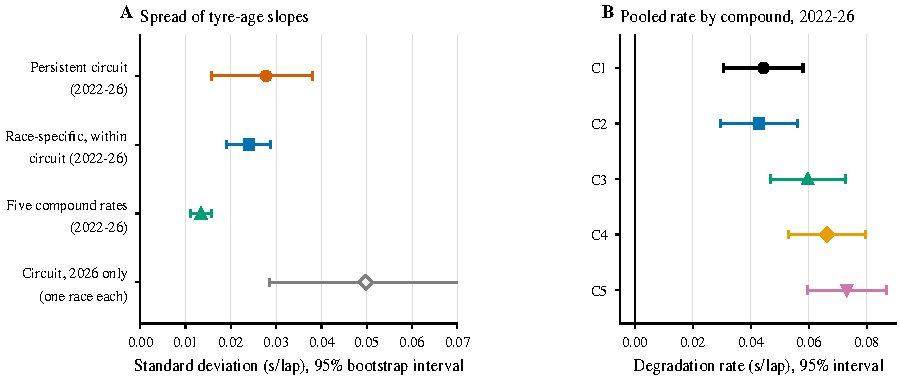
\includegraphics[width=\linewidth]{figures/fig_circuit_decomposition.pdf}
\caption{(A) Standard deviation of the tyre-age slope: persistent circuit and race-specific (event within circuit) components from the pooled 2022--26 model, the standard deviation of the five pooled compound rates, and the circuit standard deviation of the 2026 model alone, in which each circuit is raced once and the two components cannot be separated. Bars are 95\% parametric-bootstrap percentile intervals. (B) Pooled race degradation rate per compound over 2022--26 with 95\% Wald intervals; the marker shapes for compounds are those of Figure~\ref{fig:circuit}.}
\label{fig:decomp}
\end{figure}

A single season gives a less clear picture.
The 2026 season alone has a circuit standard deviation of \CircuitSD\spl{} (profile interval [\CircuitSDLo, \CircuitSDHi]; bootstrap [\CircuitSDBootLo, \CircuitSDBootHi], as in Figure~\ref{fig:decomp}A), larger than either pooled component because each 2026 circuit was raced once, so its slope mixes persistent and race-specific variation.
Its compound rates, from Eq.~\eqref{eq:race} on \NLapsRaceFit{} laps in \NRunsRaceFit{} runs by \NDriversRaceFit{} drivers at \NCircuitsRaceFit{} circuits (Figure~\ref{fig:circuit}A, Appendix Table~\ref{tab:rates}), run from \RateCTwo\spl{} (C2) to \RateCFour\spl{} (C4), with a standard deviation of \CompoundRateSD\spl{} that is no larger than sampling noise alone would produce.
C3 degrades faster than C2, by \SixConThreeTwo\spl{} [\SixConThreeTwoLo, \SixConThreeTwoHi], and C4 faster than C3, by \SixConFourThree{} [\SixConFourThreeLo, \SixConFourThreeHi], but C5 degrades more slowly than C4 (\ContrastCFiveCFour\spl{} [\ContrastCFiveCFourLo, \ContrastCFiveCFourHi]), and C1 and C2 cannot be told apart.
The order also varies between seasons.
Within the same race, softer compounds degrade faster in 2022 (\TrendSeasonTwentyTwo\spl{} per step softer [\TrendSeasonTwentyTwoLo, \TrendSeasonTwentyTwoHi]), 2023 and 2025, but not detectably in 2024 or 2026 (\WithinEventTrend\spl{} [\WithinEventTrendLo, \WithinEventTrendHi]; Appendix Table~\ref{tab:seasons}).
We do not know why the soft end of 2026 differs; candidates are compound-by-phase pace offsets, selection into who stays out, and the 2026 regulations.

\begin{figure}[t]
\centering
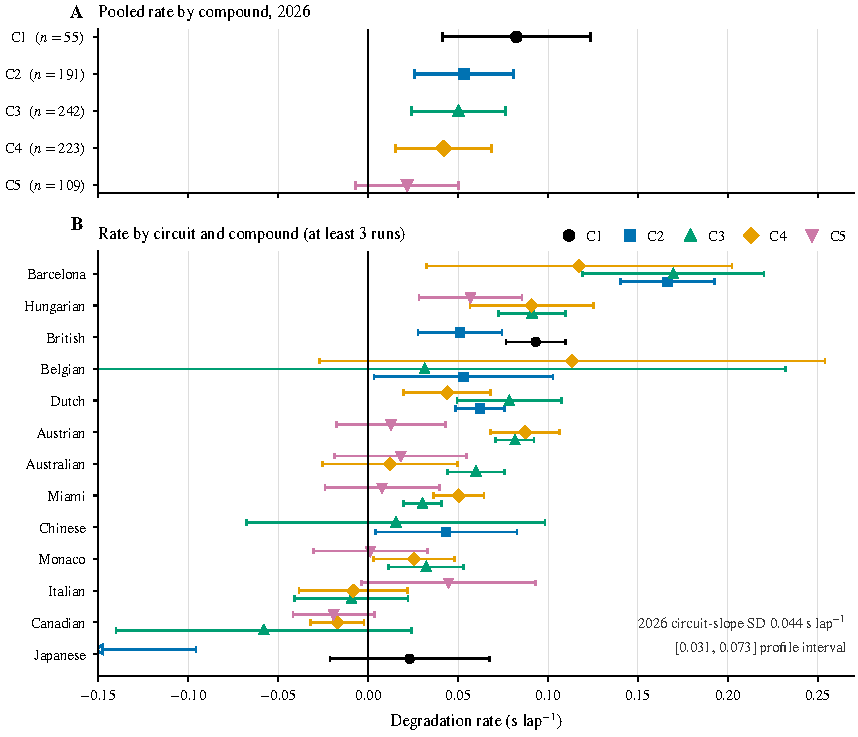
\includegraphics[width=\linewidth]{figures/fig_circuit_rates.pdf}
\caption{(A) Pooled race degradation rate per compound in 2026 with 95\% intervals; $n$ is the number of runs. (B) Separate fits for each circuit and compound with at least three runs, with 95\% run-clustered intervals, circuits ordered by mean rate. Markers: C1 circle, C2 square, C3 upward triangle, C4 diamond, C5 downward triangle. The axis is truncated: intervals are clipped at its edges, and an estimate beyond an edge is shown as an open arrowhead there. The annotation gives the 2026 circuit-slope standard deviation with its 95\% profile-likelihood interval; each circuit is raced once, so it mixes persistent and race-specific variation.}
\label{fig:circuit}
\end{figure}

Without adjustment the estimates are not just noisier but wrong in sign.
A naive regression of lap time on tyre age, with no controls, gives negative degradation for C1, C3 and C5 (\NaiveCOne, \NaiveCThree{} and \NaiveCFive\spl).
A regression that corrects for fuel within runs comes much closer, differing from Eq.~\eqref{eq:race} by \AblGapCThree\spl{} at C3 to \AblGapCOne\spl{} at C1, so most of the gain over the naive fit comes from controlling fuel and run (Appendix~\ref{app:ablation}).
In the recovery study, where the truth is known, the fuel-corrected estimator understates degradation by \RecFuelExoBiasAbs\spl{} on average even with the correct fuel constant, whereas Eq.~\eqref{eq:race} is within 0.002\spl{} of the truth on average when stops are random or depend on car pace; when stops are triggered by wear, both understate it, Eq.~\eqref{eq:race} by \RecExactWearBiasAbs\spl{} (Appendix~\ref{app:recovery}).

\subsection{Calibration of the intervals}\label{sec:calib}

The intervals are close to calibrated, though somewhat narrow for a new circuit, and only because they count runs and circuits rather than laps.
Treating laps as independent and omitting circuit slopes gives intervals only \WidthNoCircuitCThree{} (C3) to \WidthNoCircuitCOne{} (C1) times as wide as the lap-level circuit model; adding run intercepts and slopes widens them further, to \WidthShippedCOne{} (C1) to \WidthShippedCThree{} (C3) times, and cuts the residual lag-1 autocorrelation within runs from \LagOneCircuitModel{} to \LagOneShipped{} (Appendix~\ref{app:inference}).
Leaving each circuit out in turn, the nominal 80\% predictive interval covers the circuit's own fitted rate in \CovEightyLOCO{} of \CovEightyN{} circuit--compound groups (\CovEightyK{} of \CovEightyN{}; Wilson 95\% interval [\CovEightyWilsonLo, \CovEightyWilsonHi]; \citealp{brown2001interval}), and the nominal 95\% interval in \CovNinetyFiveLOCO; without the circuit variance, 80\% coverage falls to \CovEightyNoCircuit.
In simulations from the fitted model, 80\% coverage is \CovEightySBC, which checks the estimator against its own model but cannot reveal misspecification.
In the recovery study, whose data-generating process differs from the model, the nominal 95\% intervals for the compound rates cover the truth in \RecExactExoCov{} and \RecExactPaceCov{} of replicates when stops are random or depend on pace (lowest compound \RecExactPaceWorstCov), and in \RecExactWearCov{} when stops are triggered by wear.

\subsection{What can public timing data separate?}\label{sec:power}

How finely the data separate compounds depends on how many races two compounds share.
From the fitted models' own standard errors, the pooled 2022--26 data would detect, with 80\% power, a gap between neighbouring compounds of \PoolMDEFourThree\spl{} (C3 against C4) to \PoolMDETwoOne\spl{} (C1 against C2), and the 2026 season alone one of \SixMDEFourThree{} to \SixMDETwoOne\spl.
The C1 against C2 pair is the weakest link in both because C1 is nominated at few races; in 2026 the two compounds ran in only six races, and a $t$ reference with that many independent races raises the limit to \SixMDETTwoOne\spl.

To see how the allocation sets these limits, we plant a compound gap in races simulated from the fitted model, refit, and apply the Wald test of Section~\ref{sec:rates}.
Under Pirelli's actual 2026 nominations the C1 against C2 pair, with our \NRunsCOneCTwo{} runs, has a minimum detectable effect of \MDERealCOneCTwo\spl{} (other pairs \MDERealCThreeCFour{} to \MDERealCFourCFive\spl; Figure~\ref{fig:power}B), and simulations that refit the variances agree (\MDESimRealCOneCTwo\spl, Monte Carlo 95\% interval [\MDESimRealCOneCTwoLo, \MDESimRealCOneCTwoHi]); the simulated runs are idealised, with 20 laps each, so these limits are lower than the fitted ones.
Raising the run-slope standard deviation by half lifts the limit to \MDERealCOneCTwoStress\spl, while the ends of the circuit interval change it by less than 0.001\spl.
A gap of \PowerEffectSize\spl, about the hard-to-medium gap reported by \citet[Table~5]{cappelloHoegh2026}, needs \PXRunsRealSix{} runs of the two compounds under the actual allocation and \PXRunsBalSix{} if both ran at every circuit; a gap of 0.02\spl{} needs \PXRunsRealTwenty{} and \PXRunsBalTwenty{} (Figure~\ref{fig:power}A).
If the compounds ran at disjoint circuits, the circuit variance would enter the contrast and no number of runs would suffice: the minimum detectable effect at \NStintsBalanced{} runs is \MDESplit\spl, and power for a gap of 0.03\spl{} cannot exceed \PXSplitCeilThirty.
At zero effect the Wald test rejects in \PXSizeBal{} (balanced) and \PXSizeReal{} (realistic) of \PXSizeReps{} replicates, close to the nominal 0.05; a more conservative $t$ reference (12 degrees of freedom) puts the C1 against C2 limit at \MDESimRealCOneCTwoT\spl.
Simulated run requirements match the analytic ones at every effect size (Figure~\ref{fig:power}A), and the \PowerStintsCappello{} runs available to a single-driver, single-race fit fall far below all of them.

\begin{figure}[t]
\centering
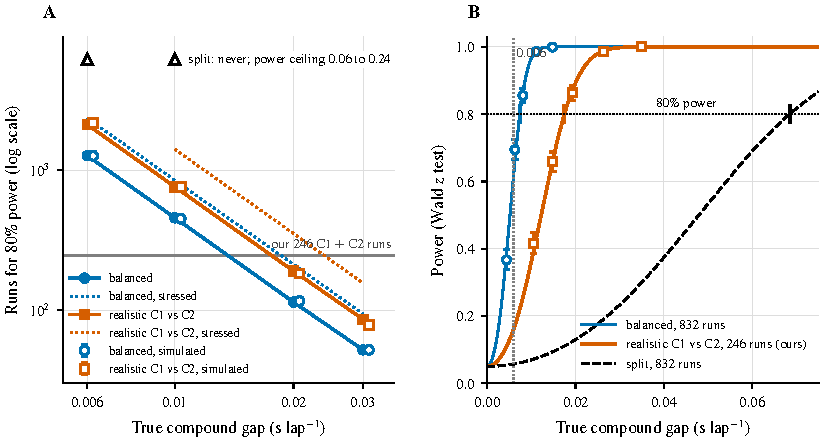
\includegraphics[width=\linewidth]{figures/fig_power.pdf}
\caption{(A) Runs of the two compared compounds needed for 80\% power against the true gap, on log axes. Solid lines are analytic (known variances): the balanced design, with both compounds at every circuit (circles), and the realistic design, Pirelli's actual 2026 nominations for C1 against C2 (squares). Dotted lines use the upper end of the circuit interval and 1.5 times the run-slope standard deviation; points beyond the grid searched are omitted. Open symbols are 80\% crossings in simulations that refit the variances and apply the Wald $z$ test (\PXSimReps{} replicates per point, up to 2{,}000 runs), with Monte Carlo 95\% intervals. The horizontal line marks our \NRunsCOneCTwo{} C1 and C2 runs. In the split design, with the compounds at disjoint circuits, power never reaches 80\% (triangles; ceiling in the label). (B) Power against the true gap at the run counts we hold: analytic curves, simulated points (\MDESimReps{} replicates each) with $\pm1.96$ Monte Carlo standard errors, and ticks at the analytic minimum detectable effect. Balanced and split curves are at \NStintsBalanced{} runs.}
\label{fig:power}
\end{figure}

\subsection{Race versus practice degradation}\label{sec:gap}

On matched used sets, races degrade less than practice, but we cannot attribute the difference to tyre management.

\textit{The gap.}\ On used sets in both settings, the pooled medium and soft race slope is \MatchedRaceSlopeMS\spl{} and the practice slope \MatchedPracticeSlopeMS\spl{} (\NMatchedCellsMS{} groups; Figure~\ref{fig:gap}A).
The gap is \LevelGapMS\spl{} [\LevelGapMSLo, \LevelGapMSHi]; it does not depend on the assumed fuel correction, which cancels in the difference.
The ratio does depend on it: under the assumed correction race degradation is \RaceToPracticeRatio{} of practice degradation (95\% bootstrap interval [\RaceToPracticeRatioLo, \RaceToPracticeRatioHi]), and Appendix~\ref{app:sens} varies the constants.
The point estimates are negative for each compound (\GapHard\spl{} for hard, \GapMedium\spl{} for medium and \GapSoft\spl{} for soft), but only the soft interval excludes zero (Appendix Table~\ref{tab:racepractice}); over all \NMatchedCellsAll{} groups in \NMatchedEventSeasons{} event-seasons the gap is \LevelGapAll\spl{} [\LevelGapAllLo, \LevelGapAllHi].
Every other design agrees in sign, with ratios from \StartAgeRatioMS{} (start-age matching) to \IntersectRatioMS{} (used sets and start age together; Figure~\ref{fig:gap}B).

The placebo shows how large a gap the design can produce by itself.
FP2 against FP1 and FP3 together, on used sets, gives \PlaceboGapMS\spl{} [\PlaceboGapMSLo, \PlaceboGapMSHi] for medium and soft over \NPlaceboCellsMS{} groups, about \PlaceboShareMS{} of the race--practice gap in size.
Subtracting it leaves \PlaceboAdjGapMS\spl{} [\PlaceboAdjGapMSLo, \PlaceboAdjGapMSHi], an interval that includes the placebo's own uncertainty and reaches zero, so differences between sessions such as run plans, fuel and conditions may explain part of the gap.

\begin{figure}[t]
\centering
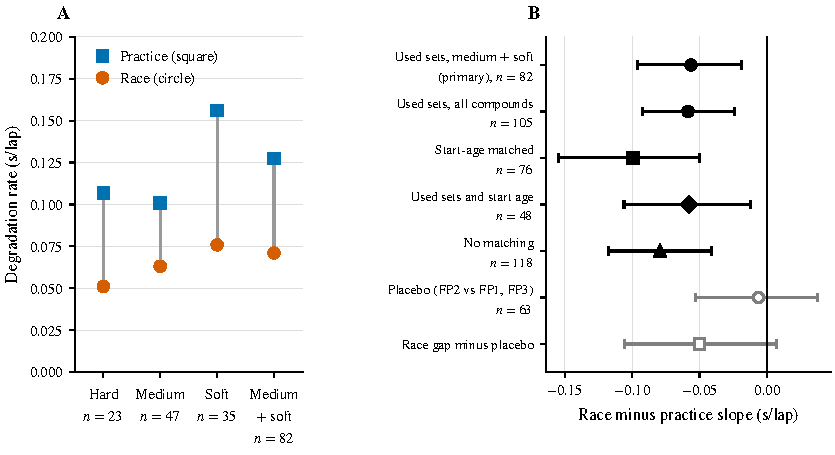
\includegraphics[width=\linewidth]{figures/fig_race_practice.pdf}
\caption{(A) Pooled race (circle) and practice (square) slopes by compound on used sets in both settings; $n$ is the number of groups. (B) Race minus practice slope with 95\% cluster-bootstrap intervals over event-seasons, for medium and soft groups unless stated: the primary design (filled circle), all compounds (filled circle), start-age matching (filled square), used sets and start age together (filled diamond), no matching (filled triangle), and the placebo comparison of FP2 with FP1 and FP3 (open circle) and the race gap minus the placebo gap (open square).}
\label{fig:gap}
\end{figure}

\textit{Is the gap tyre management?}\ The data do not show that it is.
If drivers manage softer tyres more, the gap should grow with softness, and it does not do so reliably, although the tests are underpowered.
In the difference in differences, soft minus hard is \DidTWFESoftHard\spl{} [\DidTWFESoftHardLo, \DidTWFESoftHardHi] over \DidTWFESoftHardNEvents{} events (permutation $p=\DidTWFESoftHardPPerm$, Holm-adjusted $p=\DidTWFESoftHardHolmP$); the other two pairs have intervals that include zero, and soft and medium barely differ, so the pattern is a step between hard and the other compounds rather than a gradient (Appendix Table~\ref{tab:racepractice}).
A uniform damping of every compound by the same factor would itself produce a gradient, because softer tyres have larger practice slopes: a factor of 0.5 implies \UniformDampingImplied\spl{} per step, against \UniformDampingObserved\spl{} observed.
The placebo also produces a gradient, with a soft-minus-medium gap of \PlaceboSoftMedium\spl{} [\PlaceboSoftMediumLo, \PlaceboSoftMediumHi] between practice sessions.

The primary test, the group-level trend of the gap on softness, gives \NursingTrend\spl{} per step [\NursingTrendLo, \NursingTrendHi] with one-sided permutation $p=\NursingPOneSided$ and two-sided $p=\NursingPTwoSided$, so its decision rule is not met.
Its minimum detectable effect at 80\% power is \NursingMDE\spl, more than twice the estimate, so the test cannot rule out an effect of that size.
Of the \MultiverseSpecs{} exploratory specifications, \MultiverseNegative{} give a negative trend and \MultiverseExcludesZero{} have intervals that exclude zero (Appendix~\ref{app:sens}).
Telemetry gives no support either (Appendix~\ref{app:tele}): tyre management predicts more lift-and-coast before braking zones in races than in practice, more so on softer compounds, but the slope of the race-minus-practice change in coasting time on softness is \TelePrimarySlope\,s per step [\TelePrimarySlopeLo, \TelePrimarySlopeHi] over \TelePrimaryNEventsTrend{} events in 2025--2026 (two-sided $p=\TelePrimaryPTwoSided$), and \TeleExtensionSlope\,s per step [\TeleExtensionSlopeLo, \TeleExtensionSlopeHi] over \TeleExtensionNEventsTrend{} events in 2023--2024, nominally in the opposite direction.

\subsection{Can practice predict race degradation?}\label{sec:transfer}

Practice forecasts beat a naive forecast but not a constant one.
Out of season, the scaled forecast has a mean absolute error of \MaeScalar\spl{} (95\% interval [\MaeScalarLo, \MaeScalarHi]) against \MaeNaive\spl{} [\MaeNaiveLo, \MaeNaiveHi] for the naive forecast and \MaeZero\spl{} for predicting zero (Figure~\ref{fig:forecast}).
A constant, the median race rate of other weekends, scores \MaeConstant\spl: the scaled forecast's error exceeds the constant's by \DiffScalarVsConstant\spl{} [\DiffScalarVsConstantLo, \DiffScalarVsConstantHi], and its difference from last season's race rate at the same circuit is \DiffScalarVsHistory\spl{} [\DiffScalarVsHistoryLo, \DiffScalarVsHistoryHi], both indistinguishable from zero.
A compound-specific factor does worse (\MaeCompound\spl), and neither a 50\% shrink towards the constant (\MaeShrink\spl) nor a stack of baselines (\MaeStack\spl) is detectably better (Appendix Table~\ref{tab:forecast}).
In 2026 the tuned error is \MaeTwentySixScalar\spl{} against \MaeTwentySixNaive\spl{} for the naive forecast; selecting the design and weights inside each training fold gives \MaeNested\spl, so tuning flatters the forecast by \NestedOptimism\spl.
Practice therefore removes most of the naive error but carries little information beyond a constant prior, and the choices made in cleaning practice runs hardly matter (Appendix~\ref{app:sens}).

\begin{figure}[t]
\centering
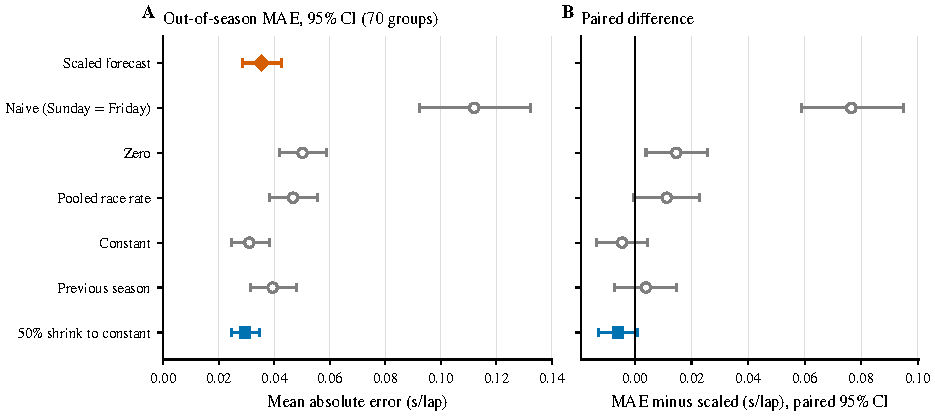
\includegraphics[width=\linewidth]{figures/fig_forecast.pdf}
\caption{Out-of-season (2022--2025) forecasts of race degradation in \HoldoutCells{} event-compound groups. (A) Mean absolute error with 95\% weekend-bootstrap intervals; (B) paired difference of each forecast's error minus the scaled forecast's, with 95\% intervals, so positive values favour the scaled forecast. The scaled forecast is the filled diamond and the 50\% shrink the filled square; all other forecasts are open circles.}
\label{fig:forecast}
\end{figure}

\subsection{Comparison with a published state-space forecaster}\label{sec:bench}

For forecasting a single driver's next lap, the state-space model of \citet{cappelloHoegh2026} is better than our pooled estimator.
Their model conditions on one driver's own history, whereas ours pools every car's laps to estimate a degradation rate; we scored both on their test laps (Appendix~\ref{app:bench}).
Over \BenchNRaces{} races the mean continuous ranked probability score (CRPS, lower is better) is \BenchCRPSSSM{} s for theirs against \BenchCRPSOurs{} s for ours, a paired difference of \BenchDiffSSM{} s [\BenchDiffSSMLo, \BenchDiffSSMHi], and ours wins \BenchWinsVsRepoSSM{} races (sign test $p=\BenchSignPSSM$).
Against their AR(1) benchmark ours wins \JournalWinsAR{} of \JournalRacesScored{} races with a CRPS difference of \JournalDiffAR{} s [\JournalDiffARLo, \JournalDiffARHi], so the two cannot be told apart.
A hierarchical state-space model with several drivers and circuit effects, as the authors suggest (p.~12), could combine both strengths.

\section{Discussion}\label{sec:discussion}

\subsection{What the results mean for analysts of public data}

Three points follow for anyone who estimates tyre degradation from public timing data.

First, circuits matter more than compounds.
Pooled over 2022 to 2026, the persistent circuit component and the race-to-race variation are each about twice the spread between compound rates; the compounds degrade in the expected order, but the within-race step from one compound to the next ranges from clearly positive in 2022 to undetectable in 2024 and 2026.
Yet last season's rate at the same circuit did not beat a constant forecast (mean absolute error \MaeHistory\spl{} against \MaeConstant\spl; Appendix Table~\ref{tab:forecast}), consistent with a race-specific component as large as the circuit one: a circuit effect that is real on average is hard to use for a single race.
A strategy model that reads a rate per compound from public lap times should therefore carry circuit- and race-level uncertainty, and naive regressions can mislead even about the sign.

Second, the data have a resolution limit that the sport's design sets.
Pirelli assigns compounds by circuit, so compound contrasts rest on the races where compounds overlap: a single season resolves neighbouring compounds only if they differ by \SixMDEFourThree{} to \SixMDETwoOne\spl, five seasons by \PoolMDEFourThree{} to \PoolMDETwoOne\spl, and with no overlap the circuit variance sets a floor that more runs at the same circuits cannot lower.
The same question arises wherever a treatment is fixed by venue, such as equipment or playing surfaces chosen per event, and simulating the actual assignment from a fitted model, as in Section~\ref{sec:power}, shows in advance what an observational comparison can deliver.

Third, practice is not a scale model of the race.
On matched used sets races degrade less than practice, by about half under the assumed fuel correction, the shortfall does not behave like a compound-specific discount, and practice adds little to a constant prior when forecasting race degradation.
For one-lap-ahead forecasts of one driver, a model that conditions on that driver's recent laps does better than our pooled estimator (Section~\ref{sec:bench}); the two answer different questions.

\subsection{Limitations}\label{sec:limits}

The analysis is observational.
Compounds differ by circuit, so a pooled fit cannot fully separate the two; we report within-race contrasts, which are free of the circuit confound, and a design analysis that shows how much the actual allocation can resolve.
The estimator assumes that, given run effects, tyre age is unrelated to unmodelled pace; if teams stop because a run's own wear is high, runs that degrade fast are cut short and the rates are understated, by \RecExactWearBiasAbs\spl{} in our simulation, with 95\% intervals that cover in only \RecExactWearCov{} of replicates.
Run means of tyre age show no sign of such dependence (Appendix~\ref{app:mundlak}), but they cannot rule it out.
The pooled fit spans a change of technical rules and tyre widths in 2026; without that season the circuit component is still the largest, but the compound spread is closer to it (Section~\ref{sec:rates}).
The persistent circuit component rests on \PooledNCircuits{} circuits with a median of \PooledEventsPerCircuit{} races each, so its share of the variance is imprecise (bootstrap [\PersistShareBootLo, \PersistShareBootHi]), and we do not identify its cause, whether surface, layout or climate.
The traffic control is endogenous, since tyre age affects traffic, and demeaning induces correlation within groups that we do not model, although intervals that allow arbitrary correlation within events are essentially no wider than ours (Appendix~\ref{app:inference}).

The race--practice comparison matches set state, tyre age and estimator, but fuel load, run plans, temperature and the purpose of a practice run are unobserved and could each contribute to the gap; the placebo bounds differences between sessions but not these.
The data do not show why race degradation is lower.
The telemetry proxies for tyre management are coarse, come from a different public source than the lap data, and are ambiguous in 2026, when power-unit energy management makes coasting routine; a null here does not show that drivers do not manage tyres.
The forecast target omits run effects and uses relative compound labels before 2026, so the evaluation measures how well practice predicts a noisy per-race estimate; the noise affects every forecast alike, but the target's selection bias could hide information that practice carries.
Finally, the state-space comparison covers \JournalRacesScored{} of the \JournalRacesTotal{} races in the published table because our cached data lack the rest.

\subsection{Extensions}

Records of the age and history of each tyre set, which teams hold, would remove the largest confound in the race--practice comparison.
More seasons with physical compound labels would sharpen the persistent share and show whether the slow-degrading C5 of 2026 persists.

\section{Conclusion}\label{sec:conclusion}

Public timing data identify persistent differences in tyre degradation between circuits, about as large as the variation from race to race and about twice the differences between compounds.
Pooled over five seasons the compounds degrade in the expected order, except that the two hardest cannot be told apart, but a single season resolves only large differences, because Pirelli's allocation lets compounds meet in few races.
On matched used tyres, races degrade less than practice, by about half under an assumed fuel correction, and the gap shows no detectable dependence on the compound.


\section*{Acknowledgements}
The code, tests, result files and manuscript source are at \url{https://github.com/akshat3144/tyre-degradation-f1}\ZenodoNote.

\section*{Data and code availability}
The data cover the 2022 to 2025 seasons and the first 13 races of 2026.
The analysis code, its tests and the result files are in the repository named in the Acknowledgements, together with the script that writes the per-event table of Pirelli compound nominations and their sources.
A script regenerates every number, table and figure in the paper from the result files, offline, and a register ties each claim to its source.
The code builds the lap tables from the FastF1 package and the OpenF1 interface; the lap tables themselves derive from the timing provider's data and remain subject to its terms, so they are not redistributed, and at the time of writing downloading the raw timing data through FastF1 requires an F1 TV account.
The code of Cappello and Hoegh carries no licence, so it is fetched by a script rather than redistributed.

\section*{Use of AI-assisted technologies}
During the preparation of this work the author used Claude (Anthropic) to assist with language editing and programming.
After using this tool, the author reviewed and edited the content as needed and takes full responsibility for the content of the publication.

\section*{Declarations}
\textbf{Funding:} none. \textbf{Conflict of interest:} the author states no conflict of interest. \textbf{Ethics:} not applicable; the study uses publicly available motorsport timing and telemetry data, with no human participants.

\appendix
\counterwithin{table}{section}
\counterwithin{figure}{section}

\section{Sensitivity and robustness}\label{app:sens}

\subsection{Compound rates and seasons}

Table~\ref{tab:rates} gives the 2026 rates behind Figure~\ref{fig:circuit}A.
Table~\ref{tab:seasons} repeats the race model for each season with weekend labels in place of physical compounds.
The circuit-slope standard deviation ranges from \CircuitSDSeasonTwentyFive{} to \CircuitSDSeasonTwentySix\spl, and the within-event compound trend has the textbook sign in 2022, 2023 and 2025 and is indistinguishable from zero in 2024 and 2026.

\begin{table}[t]
\centering\small
\begin{tabular}{@{}lrrrr@{}}
\toprule
Compound & Runs & Laps & Rate (s/lap) & 95\% interval \\
\midrule
C1 & 55 & 801 & 0.0410 & [0.0079, 0.0742] \\
C2 & 191 & 2{,}836 & 0.0373 & [0.0081, 0.0665] \\
C3 & 242 & 3{,}316 & 0.0544 & [0.0258, 0.0830] \\
C4 & 223 & 2{,}943 & 0.0633 & [0.0346, 0.0921] \\
C5 & 109 & 1{,}143 & 0.0385 & [0.0090, 0.0680] \\
\midrule
2026 circuit-slope SD (13 circuits, one race each) &  &  & 0.0498 & [0.0354, 0.0810] \\
SD of the five compound rates &  &  & 0.0114 &  \\
Within-event trend per step softer &  &  & \ensuremath{-}0.0010 & [\ensuremath{-}0.0047, \ensuremath{+}0.0028] \\
\bottomrule
\end{tabular}

\caption{Race degradation rate per compound in 2026 (seconds lost per lap of tyre age) from the mixed model of Eq.~\eqref{eq:race}, with 95\% Wald intervals. The circuit-slope standard deviation has a 95\% profile-likelihood interval. The last row is the within-event trend per step from a harder to a softer compound, estimated with one fixed slope per event (negative means softer compounds degrade more slowly within the same race).}
\label{tab:rates}
\end{table}

\begin{table}[t]
\centering\small
\begin{tabular}{@{}lrrl@{}}
\toprule
Season & Circuits & Circuit-slope SD (s/lap) & Within-event trend per step softer \\
\midrule
2022 & 18 & 0.0430 & \ensuremath{+}0.0109 [0.0040, 0.0179] \\
2023 & 16 & 0.0309 & \ensuremath{+}0.0024 [\ensuremath{-}0.0046, 0.0095] \\
2024 & 18 & 0.0258 & \ensuremath{+}0.0001 [\ensuremath{-}0.0064, 0.0065] \\
2025 & 17 & 0.0235 & \ensuremath{+}0.0048 [\ensuremath{-}0.0031, 0.0127] \\
2026 & 13 & 0.0439 & \ensuremath{-}0.0112 [\ensuremath{-}0.0177, \ensuremath{-}0.0048] \\
\bottomrule
\end{tabular}

\caption{Race model by season with hard, medium and soft labels in place of the physical compounds of Table~\ref{tab:rates}, so the 2026 row differs slightly from it (circuit-slope SD and within-event trend). The within-event trend is the change in degradation rate (s/lap) per step from a harder to a softer label with one slope per event, with a 95\% Wald interval; positive is the textbook sign.}
\label{tab:seasons}
\end{table}

\subsection{Inference under alternative error structures}\label{app:inference}

Table~\ref{tab:inference} gives the width of the 95\% interval for each 2026 compound rate under six ways of counting independent information.
Treating laps as independent produces the narrowest intervals; circuit slopes, run intercepts and run slopes each widen them and reduce the residual autocorrelation within runs.
The last two rows use fixed-effects regressions with cluster-robust errors, which allow any correlation within a run or within an event, including the correlation that demeaning induces.
Clustering by event, with a $t$ reference on 12 degrees of freedom, gives intervals narrower than ours for every compound, so the correlation we do not model does not make our intervals too narrow.

\begin{table}[t]
\centering\footnotesize\setlength{\tabcolsep}{4pt}
\begin{tabular}{@{}lrrrrrr@{}}
\toprule
Inference & C1 & C2 & C3 & C4 & C5 & Lag-1 autocorr. \\
\midrule
Laps independent, no circuit slope & 0.025 & 0.011 & 0.007 & 0.008 & 0.011 & -- \\
Laps independent, circuit slope & 0.053 & 0.042 & 0.040 & 0.041 & 0.042 & 0.36 \\
Circuit slope, run intercepts & 0.069 & 0.048 & 0.046 & 0.047 & 0.048 & 0.26 \\
Circuit slope, run intercepts and slopes (ours) & 0.082 & 0.055 & 0.052 & 0.053 & 0.057 & 0.23 \\
Fixed effects, errors clustered by run & 0.023 & 0.021 & 0.014 & 0.016 & 0.031 & -- \\
Fixed effects, errors clustered by event, $t_{12}$ & 0.024 & 0.056 & 0.032 & 0.044 & 0.053 & -- \\
\bottomrule
\end{tabular}

\caption{Width of the 95\% interval (s/lap) for each 2026 compound rate under alternative inference. The first four rows are mixed models of Eq.~\eqref{eq:race} with progressively more random effects; ``ours'' is the specification used throughout. The last two rows are regressions with driver-in-event fixed effects and cluster-robust standard errors; they omit the circuit and run terms, so their point estimates differ from the mixed models (for C4 and C5 by about half) and only their widths are compared here. The last column is the residual lag-1 autocorrelation within runs, where defined.}
\label{tab:inference}
\end{table}

\subsection{Why a cross-sectional race estimator fails}\label{app:xs}

A cross-sectional alternative to Eq.~\eqref{eq:race} regresses lap time on tyre age within each event, lap and compound, with no run terms.
It compares cars of different tyre age on the same lap, but who is on older tyres depends on pit timing, which depends on strategy and car pace, so tyre age is correlated with unmodelled pace.
The estimator returns negative soft slopes, and for the race-only trend across compounds it gives \ReconCrossSectionalAll\spl{} per step over all seasons.
Run intercepts in Eq.~\eqref{eq:race} absorb each run's pace level, so the slope is no longer driven by who has stopped.
We therefore do not interpret the cross-sectional estimate.

The sign of the race-only trend across compounds depends on how the slope is identified.
Within-run contrasts, which compare a car with itself, give \ReconWithinRunAll\spl{} per step softer [\ReconWithinRunAllLo, \ReconWithinRunAllHi] over all seasons, and the race contrasts of the fixed-effects design in Table~\ref{tab:racepractice} are about \DidTWFESoftHardRaceContrast\spl{} between each pair of compounds.
A field-demeaned slope without run terms, which compares cars with each other on the same lap, gives \ReconFieldDemeanedAll\spl{} on the same groups, the sign error that run terms remove.
The two kinds of design answer different questions, and the fixed-effects race contrasts are means over only the events that have practice sessions.

\subsection{Exploratory specifications for the management test}

The analysis of race against practice has many analyst choices \citep{gelman2014crisis}.
As an exploratory check, we re-ran the trend test of Section~\ref{sec:gap} over \MultiverseSpecs{} alternative specifications that vary the assumed fuel burn (1.4, 1.7 and 2.0\,kg per lap) and fuel effect (0.025, 0.033 and 0.040\,s/kg), the tyre-age window, run length, the minimum number of runs per group, whether sprints count as practice, the season set and the race estimator.
\MultiverseNegative{} of \MultiverseSpecs{} trends are negative and \MultiverseExcludesZero{} have bootstrap intervals that exclude zero.
Because the same fuel constant is added to every slope, it leaves the trend and the gap unchanged and moves only levels and ratios.

\subsection{Practice design choices}

Practice runs are cleaned by choices that could affect the forecast of Section~\ref{sec:transfer}.
Out of season, keeping runs bridged across short gaps changes MAE by \KeepRunsDiff\spl{} relative to the main frame [\KeepRunsDiffLo, \KeepRunsDiffHi] over \KeepRunsCommonCells{} groups (negative means the variant is better), and in 2026 trimming the warm-up lap changes it by \WarmupDiff\spl{} [\WarmupDiffLo, \WarmupDiffHi] (sign-flip $p=\WarmupSignFlipP$).
The main frame has \PracticeLapsShipped{} laps against \PracticeLapsLegacy{} for the earlier design.
The choices make small differences that we do not treat as evidence for any one design.

\subsection{Naive and fuel-corrected estimators}\label{app:ablation}

Figure~\ref{fig:sign} compares three estimators of the 2026 race rates on the same laps: the naive regression, the fuel-corrected regression within runs and the adjusted model of Eq.~\eqref{eq:race}.
The naive regression has the wrong sign for C1, C3 and C5 (\NaiveCOne, \NaiveCThree{} and \NaiveCFive\spl) and \NaiveCTwo\spl{} for C2, consistent with tyre age being confounded with fuel burn, pit-stop timing and traffic.
The fuel-corrected regression is much closer to the adjusted model, differing from it by \AblGapCThree\spl{} at C3 and \AblGapCOne\spl{} at C1.
The remaining difference may reflect track evolution and traffic, which the fuel-corrected regression does not control.

\begin{figure}[t]
\centering
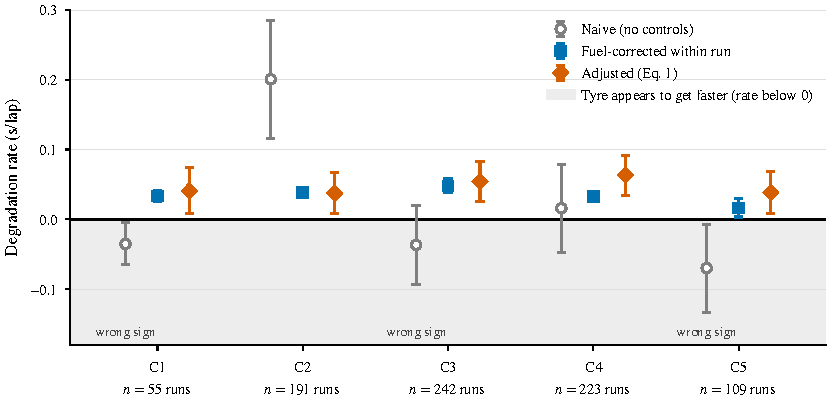
\includegraphics[width=\linewidth]{figures/fig_sign_error.pdf}
\caption{Race degradation rate per compound in 2026 under three estimators applied to the same laps: naive (open circle), fuel-corrected within runs (filled square) and adjusted, Eq.~\eqref{eq:race} (filled diamond). Markers are estimates and bars 95\% intervals (run-clustered for the naive and fuel-corrected estimators, Wald for the mixed model). Rates below zero, marked by the shaded band, mean that the tyre appears to get faster with age; $n$ is the number of runs.}
\label{fig:sign}
\end{figure}

\subsection{Race versus practice under every design}

Table~\ref{tab:racepractice} lists the gap for each compound under the primary used-set design, the other designs, the placebo and the compound contrasts behind the management test.

\begin{table}[t]
\centering\footnotesize\setlength{\tabcolsep}{3pt}
\begin{tabular}{@{}lrrrllr@{}}
\toprule
 & $n$ & Race & Practice & Difference [95\% CI] & Ratio [95\% CI] & $p$ (Holm) \\
\midrule
\multicolumn{7}{@{}l}{\textit{Used sets in both contexts (primary): 105 groups, 67 event-seasons}} \\
Hard & 23 & 0.051 & 0.107 & \ensuremath{-}0.056 [\ensuremath{-}0.116, 0.005] & 0.48 [0.20, 1.10] &  \\
Medium & 47 & 0.063 & 0.101 & \ensuremath{-}0.038 [\ensuremath{-}0.084, 0.009] & 0.63 [0.37, 1.15] &  \\
Soft & 35 & 0.076 & 0.156 & \ensuremath{-}0.080 [\ensuremath{-}0.142, \ensuremath{-}0.026] & 0.49 [0.22, 0.79] &  \\
Medium + soft & 82 & 0.071 & 0.127 & \ensuremath{-}0.056 [\ensuremath{-}0.096, \ensuremath{-}0.019] & 0.56 [0.36, 0.81] &  \\
All & 105 & 0.067 & 0.125 & \ensuremath{-}0.059 [\ensuremath{-}0.093, \ensuremath{-}0.024] & 0.53 [0.36, 0.75] &  \\
\midrule
\multicolumn{7}{@{}l}{\textit{Other designs, medium + soft}} \\
Start-age matched & 76 & 0.060 & 0.159 & \ensuremath{-}0.099 [\ensuremath{-}0.154, \ensuremath{-}0.050] & 0.38 [0.12, 0.62] &  \\
Used sets, start-age matched & 48 & 0.090 & 0.147 & \ensuremath{-}0.058 [\ensuremath{-}0.106, \ensuremath{-}0.012] & 0.61 [0.39, 0.90] &  \\
No matching & 118 & 0.059 & 0.139 & \ensuremath{-}0.079 [\ensuremath{-}0.118, \ensuremath{-}0.041] & 0.43 [0.29, 0.61] &  \\
\midrule
\multicolumn{7}{@{}l}{\textit{Placebo: practice 2 (first column) against practice 1 and 3, used sets}} \\
Medium + soft & 63 & 0.150 & 0.156 & \ensuremath{-}0.006 [\ensuremath{-}0.053, 0.037] & 0.96 [0.72, 1.32] &  \\
All & 76 & 0.148 & 0.152 & \ensuremath{-}0.003 [\ensuremath{-}0.049, 0.038] & 0.98 [0.75, 1.34] &  \\
Gap minus placebo gap &  &  &  & \ensuremath{-}0.050 [\ensuremath{-}0.106, 0.007] &  &  \\
\midrule
\multicolumn{7}{@{}l}{\textit{Compound slope contrast per context, and difference in differences, per event}} \\
Soft $-$ hard & 21 & \ensuremath{+}0.018 & \ensuremath{+}0.089 & \ensuremath{-}0.071 [\ensuremath{-}0.134, \ensuremath{-}0.013] &  & 0.028 (0.085) \\
Soft $-$ medium & 32 & \ensuremath{+}0.018 & \ensuremath{+}0.017 & \ensuremath{-}0.006 [\ensuremath{-}0.048, 0.035] &  & 0.807 (0.807) \\
Medium $-$ hard & 31 & \ensuremath{+}0.018 & \ensuremath{+}0.064 & \ensuremath{-}0.040 [\ensuremath{-}0.085, 0.005] &  & 0.091 (0.182) \\
\bottomrule
\end{tabular}

\caption{Race and practice degradation. Italic rows are panel headings. The primary design keeps used sets in both settings; its panel lists each compound, medium and soft together (\NMatchedCellsMS{} groups, the headline in the text) and all compounds (\NMatchedCellsAll{} groups). In the first three panels $n$ is the number of race--compound groups; Race and Practice are pooled slopes (s/lap), the difference is race minus practice and the ratio is race over practice, with 95\% percentile cluster-bootstrap intervals over event-seasons. In the placebo panel the first slope column is FP2 and the second is FP1 and FP3 together. The row ``Gap minus placebo gap'' is for medium and soft, with a joint-bootstrap interval. In the last panel $n$ is the number of events, the two slope columns are the mean race and practice contrasts between the named compounds, the difference is the mean difference in differences with its 95\% bootstrap interval, and the last column is the two-sided sign-flip permutation $p$-value with its Holm-adjusted value in parentheses.}
\label{tab:racepractice}
\end{table}

\section{Checks on the race estimator}\label{app:checks}

\subsection{Exact and approximate demeaning}\label{app:exact}

Eq.~\eqref{eq:race} demeans every fixed-effect column within the (event, lap) group: the compound indicators $\tilde D_{c}$, with one compound as the reference, and their products with raw tyre age, $\widetilde{(D_c a)}$.
Our first analysis instead used the raw indicators for the offsets and the indicator times tyre age demeaned over all cars, $D_c\,\tilde a$, for the slopes.
The two coincide when every car on a lap uses the same compound, which is rare in a race.
When compounds are mixed, $D_c\,\tilde a$ measures a car's tyre age against cars on other compounds, so it carries part of the other compounds' offsets and slopes, and the error falls hardest on compounds that run at few races or alongside many others.
Table~\ref{tab:exact} fits both constructions to the same laps with the same random effects and the same REML engine.
In 2026 the approximate construction roughly doubles the C1 rate and halves the C5 rate, which reverses the apparent order of the compounds; pooled over 2022--26 it compresses the five rates towards each other, cutting their standard deviation from \PooledCompoundSD{} to \ApproxPoolCompoundSD\spl, while the circuit component moves less (\PersistSD{} against \ApproxPoolCircuitSD\spl).
In the recovery study below, the approximate construction is biased for the compound at the edge of the allocation (C1 by about 0.013\spl) even when stops are random, and the exact one is not.

\begin{table}[t]
\centering\footnotesize\setlength{\tabcolsep}{4pt}
\begin{tabular}{@{}lrrrrrrr@{}}
\toprule
Fit & C1 & C2 & C3 & C4 & C5 & Compound SD & Circuit SD \\
\midrule
2026, exact & 0.041 & 0.037 & 0.054 & 0.063 & 0.039 & 0.0114 & 0.0498 \\
2026, approximate & 0.082 & 0.053 & 0.050 & 0.042 & 0.022 & 0.0219 & 0.0437 \\
2022--26 pooled, exact & 0.044 & 0.043 & 0.060 & 0.066 & 0.073 & 0.0134 & 0.0278 \\
2022--26 pooled, approximate & 0.056 & 0.047 & 0.058 & 0.059 & 0.053 & 0.0047 & 0.0247 \\
\bottomrule
\end{tabular}

\caption{Race degradation rate per compound (s/lap) under the exact demeaning of Eq.~\eqref{eq:race} and the approximate construction $D_c\,\tilde a$, on the same laps with the same random effects. Compound SD is the standard deviation of the five rates; circuit SD is the circuit-slope standard deviation (2026) or its persistent component (pooled).}
\label{tab:exact}
\end{table}

\subsection{Recovery of known rates}\label{app:recovery}

Each replicate simulates the 13 races of 2026 with their actual compound nominations, 20 cars and 55 laps.
Lap time is the sum of car pace, a fuel effect, track evolution that differs by race, a weather shock shared by the field, a compound offset, a tyre-age slope made of the compound rate plus circuit and run deviations, a run intercept and serially correlated noise; the variance components are close to the fitted 2026 values, and the planted compound rates span 0.02 to 0.08\spl.
There are no safety cars, retirements or traffic, which favours every estimator.
Each car makes one or two stops.
Stops fall at random laps (random), earlier and more often for slower cars (pace), or when the lap time a run has lost since its stop crosses a threshold, so that runs that degrade fast end early (wear).
All three scenarios share every random draw except the stop laps, and each has \RecReps{} replicates.

Table~\ref{tab:recovery} reports the mean bias over compounds, the mean absolute bias and the coverage of nominal 95\% intervals.
The naive regression is biased low by 0.06 to 0.08\spl{} in every scenario.
The fuel-corrected regression is biased low by \RecFuelExoBiasAbs\spl{} even with the right fuel constant, because track evolution is confounded with tyre age within a run.
The cross-sectional and field-demeaned regressions, which compare cars on the same lap without run terms, are unbiased when stops are random but have bias \RecCrossPaceBias\spl{} when slower cars stop earlier, the selection that run terms absorb.
Eq.~\eqref{eq:race} has mean absolute bias below 0.002\spl{} in both of those scenarios, with coverage \RecExactExoCov{} and \RecExactPaceCov, a little below the nominal level.
When stops are triggered by wear the identifying assumption fails, and Eq.~\eqref{eq:race} understates the rates by \RecExactWearBiasAbs\spl{} with coverage \RecExactWearCov; adding run means (Section~\ref{app:mundlak}) reduces this only slightly.
The circuit-slope standard deviation, planted at \RecTrueCircuitSD\spl, is recovered with bias \RecExactExoCircBias{} and \RecExactPaceCircBias\spl, and \RecExactWearCircBias\spl{} under wear-triggered stops.
The expectations for the first estimators were written before the first run; those for the corrected estimator were added after the correction, and the coverage band we set for it (0.925 to 0.975) is narrowly missed.

\begin{table}[t]
\centering\scriptsize\setlength{\tabcolsep}{3pt}
\begin{tabular}{@{}lrrrrrrrrr@{}}
\toprule
\multicolumn{1}{l}{} & \multicolumn{3}{c}{Random stops} & \multicolumn{3}{c}{Stops by pace} & \multicolumn{3}{c}{Stops by wear} \\
\cmidrule(lr){2-4}\cmidrule(lr){5-7}\cmidrule(l){8-10}
Estimator & Bias & $|$Bias$|$ & Cov. & Bias & $|$Bias$|$ & Cov. & Bias & $|$Bias$|$ & Cov. \\
\midrule
Naive & \ensuremath{-}0.062 & 0.062 & 0.05 & \ensuremath{-}0.077 & 0.077 & 0.02 & \ensuremath{-}0.070 & 0.070 & 0.03 \\
Fuel-corrected within run & \ensuremath{-}0.012 & 0.012 & 0.42 & \ensuremath{-}0.012 & 0.012 & 0.43 & \ensuremath{-}0.029 & 0.029 & 0.22 \\
Cross-sectional, no run terms & \ensuremath{+}0.000 & 0.000 & 0.79 & \ensuremath{-}0.027 & 0.027 & 0.51 & \ensuremath{-}0.032 & 0.032 & 0.32 \\
Field-demeaned, no run terms & \ensuremath{+}0.000 & 0.000 & 0.80 & \ensuremath{-}0.027 & 0.027 & 0.51 & \ensuremath{-}0.035 & 0.035 & 0.30 \\
Eq.~(1), approximate demeaning & \ensuremath{+}0.002 & 0.005 & 0.92 & \ensuremath{+}0.001 & 0.005 & 0.92 & \ensuremath{-}0.007 & 0.007 & 0.87 \\
Eq.~(1) (ours) & \ensuremath{+}0.000 & 0.000 & 0.92 & \ensuremath{-}0.001 & 0.001 & 0.92 & \ensuremath{-}0.009 & 0.009 & 0.79 \\
Eq.~(1) with run means & \ensuremath{+}0.000 & 0.000 & 0.92 & \ensuremath{-}0.001 & 0.001 & 0.92 & \ensuremath{-}0.008 & 0.008 & 0.81 \\
\bottomrule
\end{tabular}

\caption{Recovery of planted compound rates in \RecReps{} simulated seasons per scenario. Bias is the mean over the five compounds of the estimate minus the truth (s/lap), $|$Bias$|$ the mean of the absolute per-compound biases and Cov.\ the mean coverage of nominal 95\% intervals. Stops occur at random laps, earlier for slower cars (pace), or when a run's accumulated loss crosses a threshold (wear).}
\label{tab:recovery}
\end{table}

\subsection{Run means of tyre age}\label{app:mundlak}

The run intercepts and slopes of Eq.~\eqref{eq:race} are assumed independent of tyre age.
Adding each run's mean of its own tyre-age regressor as a fixed covariate, one per compound, lets the slopes rest on variation within runs only \citep[pp.~1056--1057]{bell2019fixed}.
The rates barely move: in 2026 the shifts range from \MundlakSixShiftThree\spl{} (C3) to \MundlakSixShiftOne\spl{} (C1), and in the pooled model they are at most \MundlakPoolShiftFive\spl, all well inside their bootstrap intervals.
A cluster-bootstrap $t$ test that the five added coefficients are zero gives $p=\MundlakSixP$ in 2026 (resampling races) and $p=\MundlakPoolP$ in the pooled model (resampling circuits), so the data show no dependence of run effects on tyre age.
The slope standard deviations change by less than 0.002\spl.
This check cannot detect selection that acts within a run, which is what wear-triggered stops create.

\section{Telemetry check of tyre management}\label{app:tele}

\subsection{Design}

If drivers manage softer tyres in races, car telemetry should show more lift-and-coast before braking zones, with the race-minus-practice increase larger on softer compounds.
The primary proxy is coasting time, defined as the unbroken stretch before a braking zone with throttle below 1\%, no braking and speed above 150\,km/h.
Secondary proxies are total coasting time, the fraction of lap time at full throttle, mean apex speed and mean braking deceleration; we apply no multiplicity correction to them and read them only as corroboration.
For each season, event and compound label we take the race-minus-practice difference in the proxy, adjusted for tyre age and, in the race, for race progress as a fuel proxy.
The race sessions are compared with FP2, the session in which race simulations run.
We regress the difference on softness with event fixed effects, and we obtain $p$-values from permuting labels within events and intervals from an event-clustered bootstrap.
Fuel saving would also raise coasting, but on every compound alike, which is why the test uses the slope on softness and not the level.

\subsection{Source and results}

The primary sample is 2025 and 2026 (\TelePrimaryEvents{} events, \TelePrimaryLaps{} laps); the exploratory extension, added after the primary result, is 2023 and 2024 (\TeleExtensionEvents{} events).
Car data came from the OpenF1 interface, because the source that FastF1 uses for car data was not accessible; the proxies and thresholds were fixed before the switch and left unchanged, and \TeleJoinFraction{} of the wanted laps in the primary sample matched our laps on lap time.
Results are in Section~\ref{sec:gap}.
Traffic, drafting, safety-car restarts and different track evolution between sessions are not controlled, and the 2026 power units make coasting a normal energy-management tool, so the proxy is not a clean tyre signal in that season.

\section{Comparison with a published state-space model}\label{app:bench}

\subsection{Method}

We ran the published Stan code of \citet{cappelloHoegh2026} \citep{carpenter2017stan} on their data and compared our pooled model with their forecasts.
Their evaluation is rolling-origin: within each run, the last quarter of laps is predicted one step ahead from all earlier laps.
We score our model on exactly their test laps, using the continuous ranked probability score (CRPS) \citep{gneiting2007scoring} and the root mean square prediction error (RMSPE), and compare per race.
Our forecaster sees every car's laps up to the origin but not the target lap: it tracks the driver's own pace level and projects it at the degradation rate fitted from the field's laps so far, with a normal predictive distribution whose spread comes from its own earlier errors.
Their state-space model uses one driver's laps only, so our model has more information.
We compare with both their state-space model and the AR(1) with resets at each new run that the journal version uses as a benchmark, over the \JournalRacesScored{} of the \JournalRacesTotal{} races of their Table~4 that our cached 2025 feed covers.

\subsection{Reproducing their estimates}

Our run of their Extension~1 model gives hard \TableThreeHard\spl{} and medium \TableThreeMedium\spl{} at the Austrian Grand Prix (published \TableThreeHardPub{} and \TableThreeMediumPub), with $P(\text{medium}>\text{hard})=\PMediumGtHard$ (Table~\ref{tab:repro}).
Their fuel ramp is indexed by retained lap rows rather than lap number and is misplaced by up to \FuelDefectKg\,kg at Austria; correcting it moves the probability to \PMediumGtHardCorrected{} and the CRPS by \FuelDefectDeltaCRPS, so the compounds still overlap.
The reproduction correlates \ReproCorr{} with the authors' per-race CRPS across \ReproRaces{} races, although most races other than Austria were re-run at fewer iterations.

\begin{table}[t]
\centering\small
\begin{tabular}{@{}llll@{}}
\toprule
Quantity & Published & Reproduced & Fuel ramp corrected \\
\midrule
Hard, $v$ (s/lap) & 0.054 [0.004, 0.133] & 0.055 [0.004, 0.132] & 0.053 [0.003, 0.130] \\
Medium, $v$ (s/lap) & 0.060 [0.009, 0.120] & 0.055 [0.007, 0.115] & 0.055 [0.007, 0.113] \\
$P(\mathrm{medium} > \mathrm{hard})$ & -- & 0.528 & 0.539 \\
\bottomrule
\end{tabular}

\caption{Degradation rates $v$ (s/lap, mean with 95\% interval) of the hard and medium compounds in the Extension~1 state-space model at the Austrian Grand Prix 2025: as published in the first version of \citet{cappello2025state} (the journal version prints 0.132 for the hard upper bound), as reproduced with their code, and with the fuel ramp indexed by lap number. $P(\mathrm{medium}>\mathrm{hard})$ is the posterior probability that the medium rate is higher.}
\label{tab:repro}
\end{table}

\subsection{Forecast comparison}

Their state-space model forecasts better (Table~\ref{tab:bench}).
On their exact test laps in \BenchNRaces{} races, our pooled model wins \BenchWinsVsRepoSSM{} races, with mean CRPS \BenchCRPSOurs{} against \BenchCRPSSSM{} and a paired difference of \BenchDiffSSM{} [\BenchDiffSSMLo, \BenchDiffSSMHi] (sign test $p=\BenchSignPSSM$).
Against their AR(1) benchmark we win \JournalWinsAR{} races, with CRPS \BenchCRPSOurs{} against \JournalCRPSAR{} (difference \JournalDiffAR{} [\JournalDiffARLo, \JournalDiffARHi], $p=\JournalSignPAR$), so we cannot be told apart from their AR(1).
Their state-space model beats its own AR(1) in \JournalSSMBeatsARCommon{} of these races on CRPS, and RMSPE gives the same order.
The tasks differ: theirs is a one-step forecast of one driver's laps from that driver's own history, ours a field-pooled degradation estimator used as a forecaster.

\begin{table}[t]
\centering\small
\begin{tabular}{@{}lrrlrr@{}}
\toprule
Comparator & Theirs & Ours & Ours minus theirs [95\% CI] & Races won & Sign test $p$ \\
\midrule
\multicolumn{6}{@{}l}{\textit{CRPS}} \\
Their state-space model & 0.220 & 0.326 & \ensuremath{+}0.106 [0.067, 0.146] & 2 of 15 & 0.0074 \\
Their AR(1) & 0.281 & 0.326 & \ensuremath{+}0.045 [\ensuremath{-}0.007, 0.095] & 5 of 15 & 0.302 \\
\multicolumn{6}{@{}l}{\textit{RMSPE}} \\
Their state-space model & 0.375 & 0.524 & \ensuremath{+}0.149 [0.093, 0.209] & 1 of 15 & 0.0010 \\
Their AR(1) & 0.456 & 0.524 & \ensuremath{+}0.068 [\ensuremath{-}0.005, 0.140] & 5 of 15 & 0.302 \\
\bottomrule
\end{tabular}

\caption{Italic rows are panel headings. Head-to-head with Cappello and Hoegh on the \BenchNRaces{} races of their Table~4 that our 2025 feed covers. Entries are means over races of the per-race score (CRPS in s, RMSPE in s), lower being better. The difference is ours minus theirs, so positive means ours is worse, with a 95\% bootstrap interval over races; races won counts races where our score is lower; the sign test is two-sided.}
\label{tab:bench}
\end{table}

\subsection{Scoring and coverage}

Their cross-validation code draws predictive samples from a skew-$t$ distribution, whereas the predictive draws in the Stan file are normal.
Scoring the skew-$t$ draws as such rather than as a normal lowers mean CRPS by \SkewTDelta{} over \SkewTRaces{} races (matched is better in \SkewTBetter), and by \SkewTAustriaDelta{} at Austria: the mismatch is real but small.
On their exact test laps our CRPS at Austria is \AustriaCRPSOurs{} against \AustriaCRPSTheirs{}, a paired lap-level difference of \AustriaDiff{} [\AustriaDiffLo, \AustriaDiffHi].
The journal's Table~4 lists \JournalRacesTotal{} races, and our cached 2025 feed covers \JournalRacesScored{} of them.
Their printed mean row for the AR(1) benchmark (\JournalPrintedMeanAR) equals the 19-race mean including Singapore (\JournalMeanARAll) although the caption says it excludes that race, so we use only the per-race rows.

\section{Forecast comparison in full}\label{app:forecast}

Table~\ref{tab:forecast} lists every practice-to-race forecast we evaluated.
The first numeric columns are out-of-season (2022 to 2025) and match Figure~\ref{fig:forecast}; the last column is 2026, where the scaled forecast is tuned on the evaluation groups and is therefore optimistic (Section~\ref{sec:transfer}).
Among the forecasts tried but not adopted, the compound-specific factor is worse and the 50\% shrink and the stack of baselines are not detectably better than the scaled forecast.

\begin{table}[t]
\centering\footnotesize
\begin{tabular}{@{}lrrlr@{}}
\toprule
Forecast & MAE & 95\% CI & MAE minus scaled & MAE, 2026 \\
\midrule
\multicolumn{5}{@{}l}{\textit{Adopted}} \\
Scaled practice forecast & 0.0355 & [0.0286, 0.0426] & -- & 0.0561 \\
\multicolumn{5}{@{}l}{\textit{Baselines}} \\
Naive (Sunday = Friday) & 0.1120 & [0.0923, 0.1324] & \ensuremath{+}0.0765 [0.0588, 0.0949] & 0.0871 \\
Zero & 0.0502 & [0.0418, 0.0590] & \ensuremath{+}0.0147 [0.0039, 0.0258] & 0.0689 \\
Pooled race rate & 0.0468 & [0.0384, 0.0556] & \ensuremath{+}0.0113 [\ensuremath{-}0.0004, 0.0229] & 0.0713 \\
Constant (other weekends' median) & 0.0311 & [0.0246, 0.0383] & \ensuremath{-}0.0045 [\ensuremath{-}0.0136, 0.0044] & 0.0726 \\
Previous season, same circuit & 0.0394 & [0.0314, 0.0480] & \ensuremath{+}0.0039 [\ensuremath{-}0.0072, 0.0149] & 0.0615 \\
\multicolumn{5}{@{}l}{\textit{Tried, not adopted}} \\
Compound-specific factor & 0.0634 & [0.0504, 0.0771] & \ensuremath{+}0.0279 [0.0161, 0.0407] & 0.0607 \\
50\% shrink toward constant & 0.0295 & [0.0245, 0.0348] & \ensuremath{-}0.0060 [\ensuremath{-}0.0129, 0.0010] & 0.0584 \\
Stack of baselines & 0.0317 & [0.0255, 0.0382] & \ensuremath{-}0.0039 [\ensuremath{-}0.0130, 0.0053] & 0.0592 \\
\bottomrule
\end{tabular}

\caption{Practice-to-race forecasts of the race degradation rate. Italic rows are panel headings. The first three numeric columns are out-of-season (2022--2025) mean absolute error (s/lap) with a 95\% weekend-bootstrap interval and the paired difference to the scaled forecast (positive favours the scaled forecast); the last column is the 2026 error, where the scaled forecast is tuned on the evaluation groups. Forecasts under ``Tried, not adopted'' were evaluated but not adopted.}
\label{tab:forecast}
\end{table}


\bibliographystyle{apalike}
\bibliography{refs}
\end{document}
